\section{Задание к курсовой работе.}
Необходимо разработать программу для численного решения уравнения конвективно-диффузионного переноса температуры в заданном поле скоростей по методу контрольного объема (МКО), применительно к задаче о течении в каверне с движущейся крышкой и с разнонагретыми стенками. Для выполнения расчета необходимо написать программу которая будет численно вычислять пространстранственные операторы по МКО и вследствии позволит разрешить уравнения конвективно-диффузионного переноса. Программа должна быть выполнена на языке программирования Fortran. Индивидуальный вариант: 3.

\section{ Порядок выполнения работы.}

\begin{enumerate}
    \item Провести расчет градиента скалярного поля $p(x,y)$ в центрах ячеек с
    помощью метода Грина-Гаусса и Грина-Гаусса с итерациями.
    \item Провести расчет дивергенции произведения скалярной величины на вектор, $div(p\cdot\vec{V})$. Расчет скалярной величины на грани необходимо провести с помощью центральной (Central), противопоточной схемы первого и второго порядка (FOU и SOU соответственно).
    \item Провести расчет лапласиана скалярного поля $p(x,y)$.
    \item Провести расчет ротора векторного поля $\vec{V}(x,y)$.
    \item Решить уравнение конвективно-диффузионного переноса скалярной величины (температуры) для заданного скалярного поля скоростей.
\end{enumerate}


\section{Описание метода конечных объемов (МКО)}
\subsection{Дискретизация уравнений.}
Метод конечных объемов (МКО) — это численный метод, который широко применяется для решения дифференциальных уравнений в частных производных. Основной особенностью метода является его способность сохранять физические законы (массу, импульс, энергию) на уровне дискретной формы уравнений, в отличие от метода конечных разностей, который работает с узловыми точками. Можно это интерпритировать так, что МКР работает с узлами и точчеными значениями, а МКО с интервалами.

Для применения МКО расчетную область делят на некоторые объемы (ячейки), которые в совокупности составляют всю исходную область. Вершины формируют узлы расчетной сетки.

Для построения контрольного объема используют один из двух методов: объемно-центрированный (Cell-centered), при котором решение ищется в центрах конечного объема, и вершино-центрированный (Vertex-based), при котором решение ищется в узлах расчетной сетки и конечные объемы строятся вокруг них (рисунок \ref{fig:1}).

\begin{figure}[H]
    \centering
    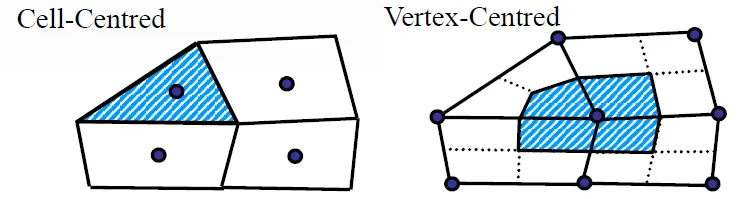
\includegraphics[width=0.75\textwidth]{img/1.png}
    \caption{Схематическое представление построения КО с помощью различных подходов.}
    \label{fig:1}
\end{figure}

Для потсроения КО рассмотрим неподвижный объем $\Omega$, изображенный на рисунке \ref{fig:2}. Поверхность КО обозначается $\sigma$, соответственно элемент поверхности и объема обозначаются как $\delta\sigma$ и $\delta\Omega$. Так для определения поток проходящих сквозь поверхность объема введем нормаль к элементарной поверхност таким образом, чтобы она была направлена наружу, тогда получим так называемый вектор элемента площадки $\delta\vec{\sigma}=\vec{n}\cdot\delta\sigma$.

\begin{figure}[H]
    \centering
    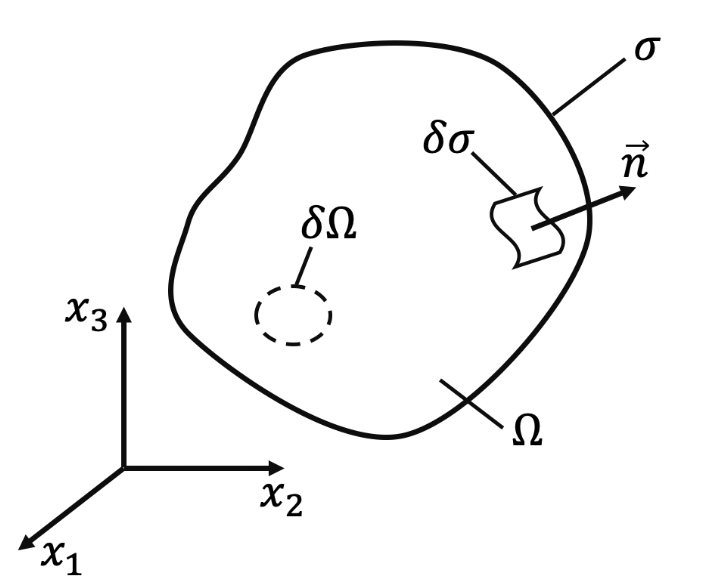
\includegraphics[width=0.5\textwidth]{img/2.png}
    \caption{Иллюстрация КО.}
    \label{fig:2}
\end{figure}

Рассмотрим задачу конвективно-диффузионного переноса скалярной величины $\phi$. Запишем уравнение описывающее этот процесс сразу в интегральной формулировке (\ref{eq:1}). Переход от интегральной формулировки к дифференциальной осуществляется путем применения теоремы Остроградского-Гаусса.

\begin{equation}
    \frac{\partial}{\partial t}\int_{\Omega}\rho\phi\delta\Omega+\oint_\sigma\vec{F}\cdot\delta\vec{\sigma} = \int_\Omega\rho S_\phi\delta\Omega
    \label{eq:1}
\end{equation}

В свою очередь вектор плотности потока $\vec{F}$ можно разложить на конвективную и диффузионную составляющие:

\begin{equation}
    \vec{F} = \vec{F}_{\text{конв}}+\vec{F}_{\text{диф}} = \rho\vec{V}\phi+\vec{q}_\phi
    \label{eq:2}
\end{equation}

Приведем континуальную форму получившихся уравнений к дискретной. Для этого введем следующие обозначения: $(...)_{c}$ - в центре ячейки, $(...)_f$ - в центре грани. Применяя теорему о среднем для объемных и поверхностных интегралов, получим:
\begin{equation}
    \frac{\partial}{\partial t} \int_\Omega\rho\phi\delta\Omega \simeq \frac{\partial(\rho\phi)_c}{\partial t}\Omega
\end{equation}
\begin{equation}
    \int_\Omega \rho S_\phi\delta\Omega \simeq (\rho S_\phi)_c\cdot\Omega
\end{equation}
Для поверхностного интеграла ввиду замкнутости мы не можем напрямую применить теорему о среднем, потому разобьем интеграл на сумму интегралов:
\begin{equation}
    \oint_\sigma\vec{F}\cdot\delta\vec{\sigma} = \sum_f\int_{\sigma_f}\vec{F}\cdot \vec{\sigma}_f\simeq \sum_f \vec{F}_f\cdot \vec{\sigma}_f
\end{equation}

В результате получаем полудискретный (ввиду того, что осталась недискретная производная по времени) аналог для уравнения конвективно-диффузионного переноса:

\begin{equation}
    \frac{\partial(\rho\phi)_c}{\partial t}\Omega+\sum_f \vec{F}_f\cdot\vec{\sigma}_f=(\rho S_\phi)_c\cdot\Omega
\end{equation}


Тогда для проведения дальнейшего расчета мы уже можем определить некоторый алгоритм или порядок действий:
\begin{enumerate}
    \item Расчет центров КО.
    \item Расчет центров граней.
    \item Расчет объем ячеек.
    \item Нахождение векторов площади грани $\vec{\sigma}_f$.
    \item Выбор способа расчет потоков $\vec{F}_f$ на грани, используя значения в центрах КО.
    \item Схема сведения задачи.
\end{enumerate}



\subsection{Описание расчета геометрических характеристик.}

Для использования МКО необходимо определить геометрические характеристики КО. Для этого рассмотрим ячейку полиэдральной формы. На рисунке \ref{fig:3} представлена ее грань. Как известно, любой многоугольник можно представь как свокоупность треугольников, таким образом разобьем грань на треугольники с вершиной в центре грани.


\begin{figure}[H]
    \centering
    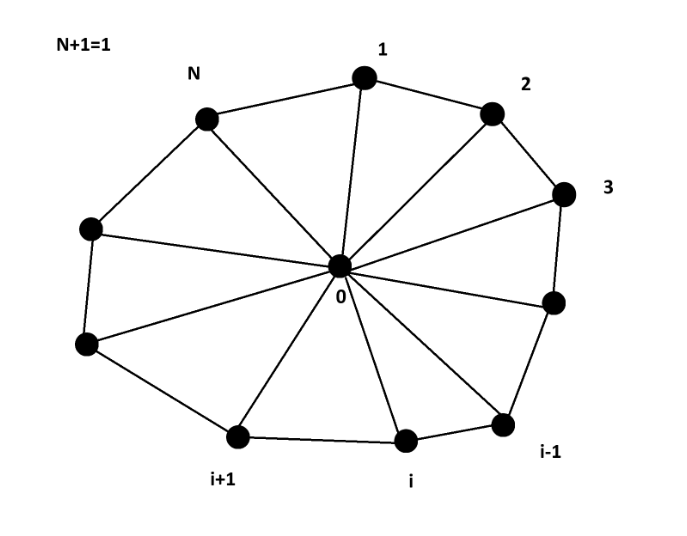
\includegraphics[width=0.55\textwidth]{img/3.png}
    \caption{Грань ячейки произвольной формы.}
    \label{fig:3}
\end{figure}

Вешины данной грани пронумерованы от 1 до N. При этом номер вершины N+1 соответствует вершине 1.

Вектор площади грани определяюется таким образом, что при разбиении на треугольники с одной из вершин в точке 0 определяется как сумма площадей данных треугольников.

\begin{equation}
    \vec{\sigma}_f=\sum_i\vec{\sigma}_{0,i,i+1} = \frac{1}{2}\sum_i(\vec{r}_0-\vec{r}_i)\times (\vec{r}_0-\vec{r}_{i+1}) = \frac{1}{2}\sum_i\vec{r}_i\times\vec{r}_{i+1}
\end{equation}

Таким образом, учитывая что индексы обходятся по кругу и тем самым уничтожают одно из слагаемых, получаем, что вектор поверхности грани не зависит от выбора точки 0. Положим, что $\vec{r}_0=\vec{r}_1$, тогда можно получить итоговую формулу для вычислений $\vec{\sigma}_f$:

\begin{equation}
    \vec{sigma}_f = \frac{1}{2}\sum_{i=2}^{N-1} (\vec{r}_1-\vec{r}_i)\times (\vec{r}_1-\vec{r}_{i+1})
\end{equation}


Для вычисления объема ячейка произвольной формы разбивается на пирамиды с основанием $\sigma_f$ и вершиной в точке 0. ТОгда можно записать:
$$\Omega = \frac{1}{3}\sum_f(\vec{r}_f-\vec{r}_0)\cdot\vec{\sigma}_f$$
Применяя теорему Остроградского-Гаусса перейдя к дискретной форме получим, что 
$$\sum_f\vec{\sigma}_f = 0$$
Тогда выражение примет вид:
\begin{equation}
    \Omega = \frac{1}{3}\sum_f \vec{r}_f\cdot\vec{\sigma}_f = \frac{1}{3}\sum_f (\vec{r}_f - \vec{r}_{f_1})\cdot\vec{\sigma}_f
\end{equation}

Последнее равенство реализует достижение вычислений одного порядка, выбрав центр произвольной грани как начало отсчета. Это позволительно ввиду отсутствия зависимости объема от точки отсчета.

Центр грани $\vec{r}_f$ определяется несколькими способами. Первый способ подразумевает вычисление путем среднего арифметического. Существуют еще способ установления центра грани в центре тяжести поверхности или центра тяжести контура. Лучшим остается последний, так как в нем отсутствует зависимость от $\vec{r}_0$. Запишем выажение для центра тяжести контура:

\begin{equation}
    \vec{r}_f = \sum_i \frac{1}{2}(\vec{r}_i+\vec{r}_{i+1})\frac{|\vec{r}_{i+1}-\vec{r}_i|}{\sum_k|\vec{r}_{k+1}-\vec{r}_k|}
\end{equation}


Последний способ определения имеет преимущество над способом
определения с помощью центра тяжести в случае вытянутой ячейки, так
как определяет более точно нормаль к поверхности, что приводит к
меньшим погрешностям при вычислении, например, диффузионных
потоков.

Аналогично для расчета центра объема: среднее арифметическое, центр тяжести, центр тяжести контура или центр тяжести каркаса. Лучшим вариантом является определения при помощи центра тяжести контура:

\begin{equation}
    \vec{r}_c = \sum_f \vec{r}_f\cdot\frac{|\vec{\sigma}_f|}{\sum_k|\vec{\sigma}_k|}
\end{equation}


Так как в данной работ рассматривается структурированная расчетная сетка с четырехугольными ячейками, вследствии чего выражения для расчетов геометрических характеристик преобразуются и сильно упрощаются.

Рассматривая двумерные расчетные сетки, каждая грань ячейки представляет собой
отрезок, а ее площадь равна длине ребра. Ввиду специфики сетки можно разбить нормали на две большие группы: грань расположенная между узлами i,j и i,j+1 ($\vec{n_{i,j}^I}$) и грань расположенная между узлами i,j и i+1,j ($\vec{n_{i,j}^J}$). Найдем общий вид формулы для этих двух вариантов. 

\begin{equation}
    \vec{r}_I = (r_{I,x}, r_{I,y}) = (x_{i,j+1} - x_{i,j}, y_{i,j+1} - y_{i,j})
\end{equation}
\begin{equation}
    \vec{n_{i,j}^I} = (r_{I,y}, -r_{I,x})
\end{equation}

Аналогично для другой группы:
\begin{equation}
    \vec{r}_J = (r_{J,x}, r_{J,y}) = (x_{i+1,j} - x_{i,j}, y_{i,j+1} - y_{i+1,j})
\end{equation}
\begin{equation}
    \vec{n_{i,j}^J} = (r_{J,y}, r_{J,x})
\end{equation}

То есть эти веткора получаются путем развороте вектора грани на 90 градусов. Тогда получим, что все нормали $\vec{n_{i,j}^I}$ будут направлены вправо, а $\vec{n_{i,j}^J}$ будут направлены вверх (на скошенных сетках нормали направлены не строго по горизонтали а как-то иначен но в направлении увеличения индекса). Схематично это представлено на рисунке \ref{fig:4}. В процессе вычисления пространственных операторов направление нормали будет выбираться таким образом, чтобы она была внешней, а это достигается путем изменения знаков в координатах вектора нормали.


\begin{figure}[H]
    \centering
    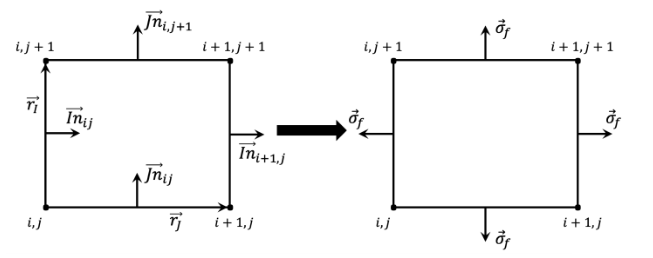
\includegraphics[width=0.75\textwidth]{img/4.png}
    \caption{Схема расположение векторов нормалей к граням.}
    \label{fig:4}
\end{figure}

Центр грани расчитывается как среднее арифметическое координат соответствующих узлов:
\begin{equation}
    \vec{r}_f = (\frac{x_{i,j+1}+x_{i,j}}{2}, \frac{y_{i,j+1}+y_{i,j}}{2}) 
\end{equation}
или
\begin{equation}
    \vec{r}_f = (\frac{x_{i+1,j}+x_{i,j}}{2}, \frac{y_{i+1,j}+y_{i,j}}{2}) 
\end{equation}

В зависимости от того какая это грань формула будет отличаться соответственно.

Центр объема в данном случае расчитывается следующим образом:

\begin{equation}
    \vec{r}_c = \sum_f \vec{r}_f \frac{\sigma_f}{\sum_k\sigma_k}
\end{equation}

В данной работе также введены фиктивные ячейки, которые имеют индексы: $i=\{0,NI\}$ при $j=\overline{1,NJ-1}$ и $j=\{0,NI\}$ при $i=\overline{1,NI-1}$. Они являются заграничными и введены для упрощения расчтов потоков для приграничных ячеек. Для рассматриваемых точек центры объемов совпадают с центрами граней с теми же индексами. Исключением является заграничные ячейки с i=0, j=0. Для них соответствующие грани имеют индексы i=1, j=1.

Объем или в данном случае площадь ячейки вычисляется, как сумма площадей двух треугольников создаваемых при проведение диоганали в четырехугольной ячейке:

\begin{equation}
    \Omega_{i,j} = \frac{1}{2}(\vec{n^I_{i,j}}\cdot\vec{r_{i,j}}+\vec{n^J_{i,j}}\cdot\vec{r_{i,j}})
\end{equation}

$$\vec{r_{i,j}} = (x_{i+1, j+1}-x_{i,j}, y_{i+1, j+1}-y_{i,j})~-~\text{Вектор диагонали}$$


\section{Описание расчета пространственных дифференциальных операторов.}
\subsection{Расчет градиента скалярной величины.}
Используя теорему Остроградского-Гаусса и теорему о среднем можем получить следующее выражение:

\begin{equation}
    \sum_f \phi_f \vec{\sigma}_f = \oint_\sigma\vec{n}\phi d\sigma = \int_\Omega \nabla\phi d\Omega \simeq (\nabla \phi)_c\Omega
\end{equation}

То есть получаем, что вычисление градиента в центре ячейки сводится к суммированию произведений значений величины на гранях и вектора грани.
Ввиду того, что мы определили объем ячейки и вектор грани, то необходимо как-то найти значение $\phi$ на грани. Для этого используется линейная интерполяция на грань: 
\begin{equation}
    \phi_f = \phi_M = (1-\beta)\phi_L+\beta\phi_R
\end{equation}

, где $\beta = \frac{|\vec{P_LM}|}{|\vec{P_LM}|+|\vec{P_RM}|}$ - весовой коэффициент.

\begin{figure}[H]
    \centering
    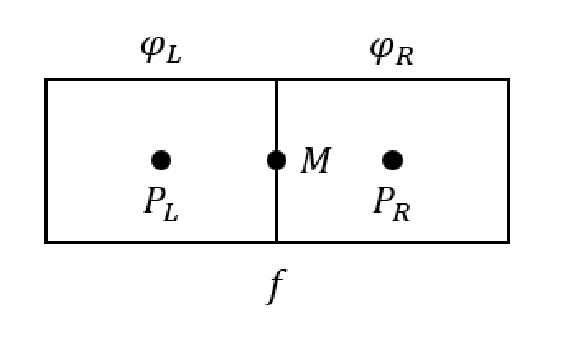
\includegraphics[width=0.55\textwidth]{img/5.png}
    \caption{Схема линейной интерполяции.}
    \label{fig:5}
\end{figure}

Для получения второго порядка точности в приграничных ячейках значение
скалярной функции в центре граничной грани b вычислялось следующим образом:

$$\phi_b = \frac{1}{2}(\phi_p+\phi_0)$$

где $\phi_P$– значение $\phi$ в центре приграничной ячейки, $\phi_0$ – значение в центре фиктивной заграничной ячейки, центр которой определялся как 
$\vec{r}_0 =  2\vec{r}_b - \vec{r}_p$ поскольку заграничная
ячейка может быть произвольной формы.

В случае скошенной расчетной сетки линейная интерполяция плохо работает и дает погрешность. Поэтому необходима применять так называемый метод Грина-Гаусса с итерациями:
\begin{equation}
    \phi_M = \phi_E + \vec{EM}\cdot(\nabla\phi)_E
\end{equation}

\begin{figure}[H]
    \centering
    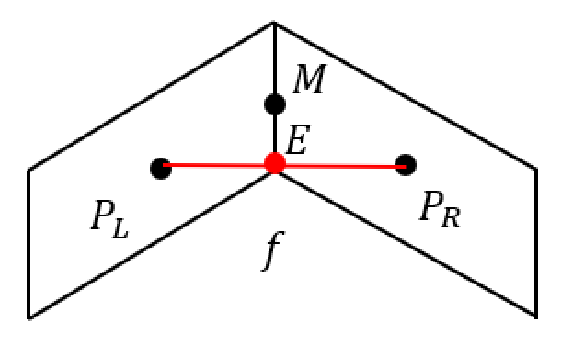
\includegraphics[width=0.55\textwidth]{img/6.png}
    \caption{Скошенная сетка.}
    \label{fig:6}
\end{figure}

Получаем итерационный процесс, где на первом шаге мы используем линейную интерполяцию на грань и поулчаем значение в точке E и считаем градиенты в центрах ячеек, а затем интерполируем линейно эти градиенты на грань и с их помощью уточняем значение в точке M пересчитывая градиенты. То есть $(\nabla\phi)_E = (1-\beta)(\nabla\phi)_L+\beta(\nabla\phi)_R.$

Таким образом итерационный процесс выглядит так, а применяя его на скошенной сетке можно улучшить значение градиентов:

\begin{equation}
    \begin{cases}
        (\nabla\phi)^k_c=\frac{1}{\Omega}\sum_f\phi^k_f\vec{\sigma}_f\\
        \phi^k_f = \phi_E+\vec{EM}\cdot(\nabla\phi)^{k-1}_E
    \end{cases}
\end{equation}


\subsubsection{Расчет дивергенции.}
Запишем теорему Остроградского-Гаусса для дивергенции произведения скалярной величины на вектор $\vec{V}$:

\begin{equation}
    \sum_f\phi_f\vec{V}_f\cdot\vec{\sigma}_f \simeq \oint_\sigma\vec{n}\cdot\phi\vec{V}d\sigma = \int_\Omega\nabla\cdot\phi\vec{V}d\Omega\simeq(\nabla\cdot\phi\vec{V})_c\cdot\Omega
\end{equation}

То есть получим:
 \begin{equation}
    (\nabla\cdot\phi\vec{V})_c = \frac{1}{\Omega}\sum_f\phi_f\vec{V}_f\cdot\vec{\sigma}_f
 \end{equation}

 Здесь для нахождения значения вектора на грани используется линеная интерполяция. Расчет скалярной величины на грани осуществаляется с помощью следующих схем:

 \begin{enumerate}
    \item Центрально разностная схема - вычисляем значения скалярной величины на грани путем линейной интерполяции:
    \item Противопоточная схема первого порядка (FOU) - при использовании данной схемы учитывается знак массового расхода $G_f = \rho\vec{V}\cdot\vec{\sigma}_f$:
    \begin{equation}
        \phi_f =
        \begin{cases}
            \phi_L,~G_f\geq 0\\
            \phi_R,~G_f<0
        \end{cases}
    \end{equation}
    \item Противопоточная схема второго порядка (SOU) также учитывает знак массового расхода
    \begin{equation}
        \phi_f =
        \begin{cases}
            \phi_L+(\nabla\phi)_L\cdot\vec{P_LM},~G_f\geq 0\\
            \phi_R+(\nabla\phi)_R\cdot\vec{P_RM},~G_f<0
        \end{cases}
    \end{equation}
 \end{enumerate}

 Для расчета скалярной величины на границах расчетной области также используеются заграничные ячейки, но уже со вторым порядком точности:
 \begin{equation}
    \phi_{f,0} = 2\phi_b-\phi_{f,1}+4(\phi_{f,1}-\phi_b)+3(\nabla\phi)_{f,1}\cdot\vec{r}_{1,b}
 \end{equation}

\subsubsection{Расчет лапласиана скалярного поля.}
Аналогично получаем:

\begin{equation}
    \int_\Omega\Delta\phi d\Omega = \oint_\sigma\frac{\partial \phi}{\partial n}d \sigma \simeq\sum_f(\frac{\partial\phi}{\partial n})_f\cdot\sigma_f = (\Delta\phi)_c\cdot\Omega
\end{equation}

Здесь необходимо найти значение производной на грани вдоль нормали и необходимо учесть поправку на неортогональость. Тогда получим:

\begin{equation}
    (\frac{\partial\phi}{\partial n})_f =\frac{\phi_R-\phi_L}{\vec{P_RP_L}}+(\vec{n}_f-\vec{i}_\xi)\cdot(\overline{\nabla\phi})_f
\end{equation}

Градиент на грани определяется путем линейной интерполяции. 

\begin{figure}[H]
    \centering
    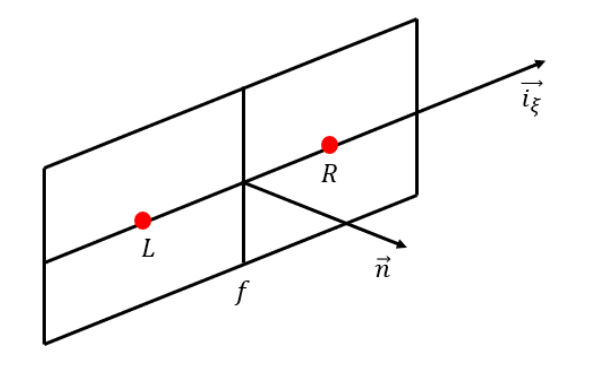
\includegraphics[width=0.55\textwidth]{img/7.png}
    \caption{Вычисление проивзодной по нормали для внутренних ячеек.}
    \label{fig:7}
\end{figure}

Для граничных ячеек с учетом поправки на неортогональность получим:
\begin{equation}
    (\frac{\partial\phi}{\partial n})_b =\frac{5}{3}\frac{\phi_1-\phi_b}{\vec{Pb}}-\frac{2}{3}\vec{n}^*\cdot({\nabla\phi})_1+(\vec{n}^*-\vec{i}_\xi)\cdot(\nabla\phi)_1
\end{equation}
\begin{figure}[H]
    \centering
    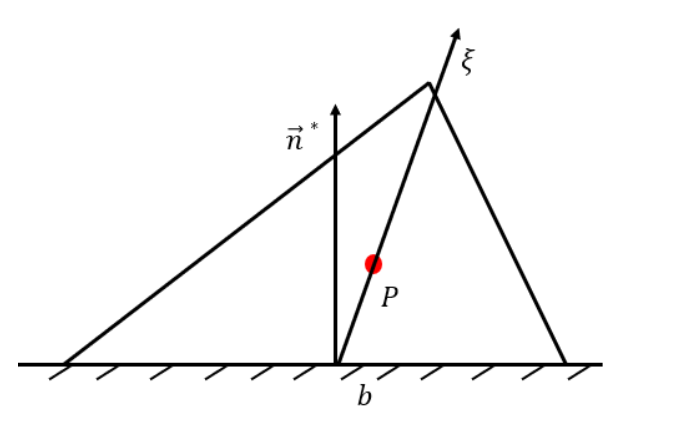
\includegraphics[width=0.55\textwidth]{img/8.png}
    \caption{Вычисление проивзодной по нормали для граничных ячеек.}
    \label{fig:8}
\end{figure}


\subsubsection{Расчет ротора векторного поля.}

Используя ту же самую теорему Гаусса-Остроградского и теорему о среднем можем получить следующее выражение аналогично:

\begin{equation}
    (\nabla\times\vec{V})_c = \frac{1}{\Omega}\sum_f\vec{V}_f\times\vec{\sigma}_f
\end{equation}

Поскольку рассматривается двумерная расчетная область, то останет только z компонента ротора, что мы можем интерпритировать как скалярную величину распределенной по расчетной области.


\section{Описание алгоритма расчета уравнения конвективно-диффузионного переноса температуры.}
В данной работе рассматривается стационарное течение несжимаемой жидкости в отсутствии объемных источников. С учтом этого уравнение конвективно-диффузионного переноса преобразуется в вид:

\begin{equation}
    \oint_\sigma(\rho\vec{V}\phi+\vec{q}_\phi)\cdot\delta\vec{\sigma} =0
\end{equation}

В качестве скалярной функции рассмтривается внутренняя энергия, тогда обозначим удельную внутреннюю энергию как $\phi=e$. Учитывая, что диффузионный поток можно определить используя базовую модель Фурье-Фика, то есть:
\begin{equation}
    \vec{q}_e = -\lambda\nabla T
\end{equation}
, где $\lambda$ - коэффициент теплопроводности, а $T$ - температура. А также взять во внимание тот факт, что внутренняя энергия связан с температурой для несжимаемой жидкости следующим соотношением: $e=c_pT$. Итоговое выражение выглядит следующим образом:

\begin{equation}
    \oint_\sigma (\rho c_pT\vec{V}-\lambda\nabla T)\cdot\delta\vec{\sigma}=0
\end{equation}

Данное уравнение можем обезразмерить, введя масштабы скорости $\vec{V}_s$, температуры $T_s$ и длины $L_s$. Тогда уравнение преобразуется в слудеющий вид:

\begin{equation}
    \oint_\sigma(T\vec{V}-\frac{\lambda}{\mu c_p}\frac{\mu}{\rho V_s L_s}\nabla T)\cdot\vec{\sigma} = \oint_\sigma(T\vec{V}-\frac{1}{Pr \cdot Re}\nabla T)\cdot\vec{\sigma} =0
\end{equation}

Получим уравнение внутренней энергии в безразмерной форме.

Полученное уравнение будем решать методом установления. Для применения
данного метода вводится псевдовремя $\tau$, а в уравнении добавляется соответствующая производная температуры по псевдовремени. Ищется стационарное решение, поэтому добавленное слагаемое проподает и получается, что исходное выражение верно.

\begin{equation}
    \int_\Omega \frac{\partial T}{\partial \tau}\delta\Omega+\oint_\sigma(T\vec{V}-\frac{1}{Pr \cdot Re}\nabla T)\cdot\vec{\sigma} =0
\end{equation}

В дискретной форме, используя явную схему Эйлера для дискретизации по вермени, обусловленной тем, что нам не важен порядок точности по этому времени, как и шаг, получим для M+1 шага по времени:

\begin{equation}
    \frac{T^{M+1}_c-T^M_c}{\Delta\tau_c} = - \frac{1}{\Omega}\sum_f(T\vec{V}-\frac{1}{Pr\cdot Re}\nabla T)^M_f\cdot\vec{\sigma}_f=R^M_c
\end{equation}

Получили формулу для невязки стационарного оператора на текущем временном слое в центре расматриваемой ячейки. Для определения невязки расчитываются конвективный и диффузионные потоки на гранях ячейки, расчет которых был представлен ранее. Шаг по псевдовремени для рассматриваемой ячейки определяется по локальному времени путем следующего соотношения:

$$ \frac{1}{\Delta \tau_c} = \frac{1}{\Delta \tau_c^\text{конв}} + \frac{1}{\Delta \tau_c^\text{дифф}}$$

$$
\Delta \tau_c^\text{конв} = \text{CFL} \frac{\Omega}{\sum_f |\mathbf{v}_f \cdot \sigma_f|}, \quad
\Delta \tau_c^\text{дифф} = \text{VNM} \frac{1}{2 \sum_f \frac{a_f}{\sigma_f}} $$

где CFL -  число Куранта, которое в случае равномерной расчетной сетки равно $CFL=V_s\frac{\Delta t}{\Delta x}$, VNM - число фон Неймана, которое в случае равномерной сетки равно $VNM=D\frac{2\Delta t}{\delta x^2}$. Их значение задаются так, чтобы достичь максимальной скорости сходимости, а устойчивость при этом сохранялась. Обычно их выбирают такими, чтобы они были меньше или равны 1.


\section{Описание алгоритма вычислительного кода.}
Блок схема для вычисления пространственных операторов и разрешения уравнений конвективно-диффузионного переноса представлена на рисунке \ref{fig:9}.

\begin{figure}[H]
    \centering
    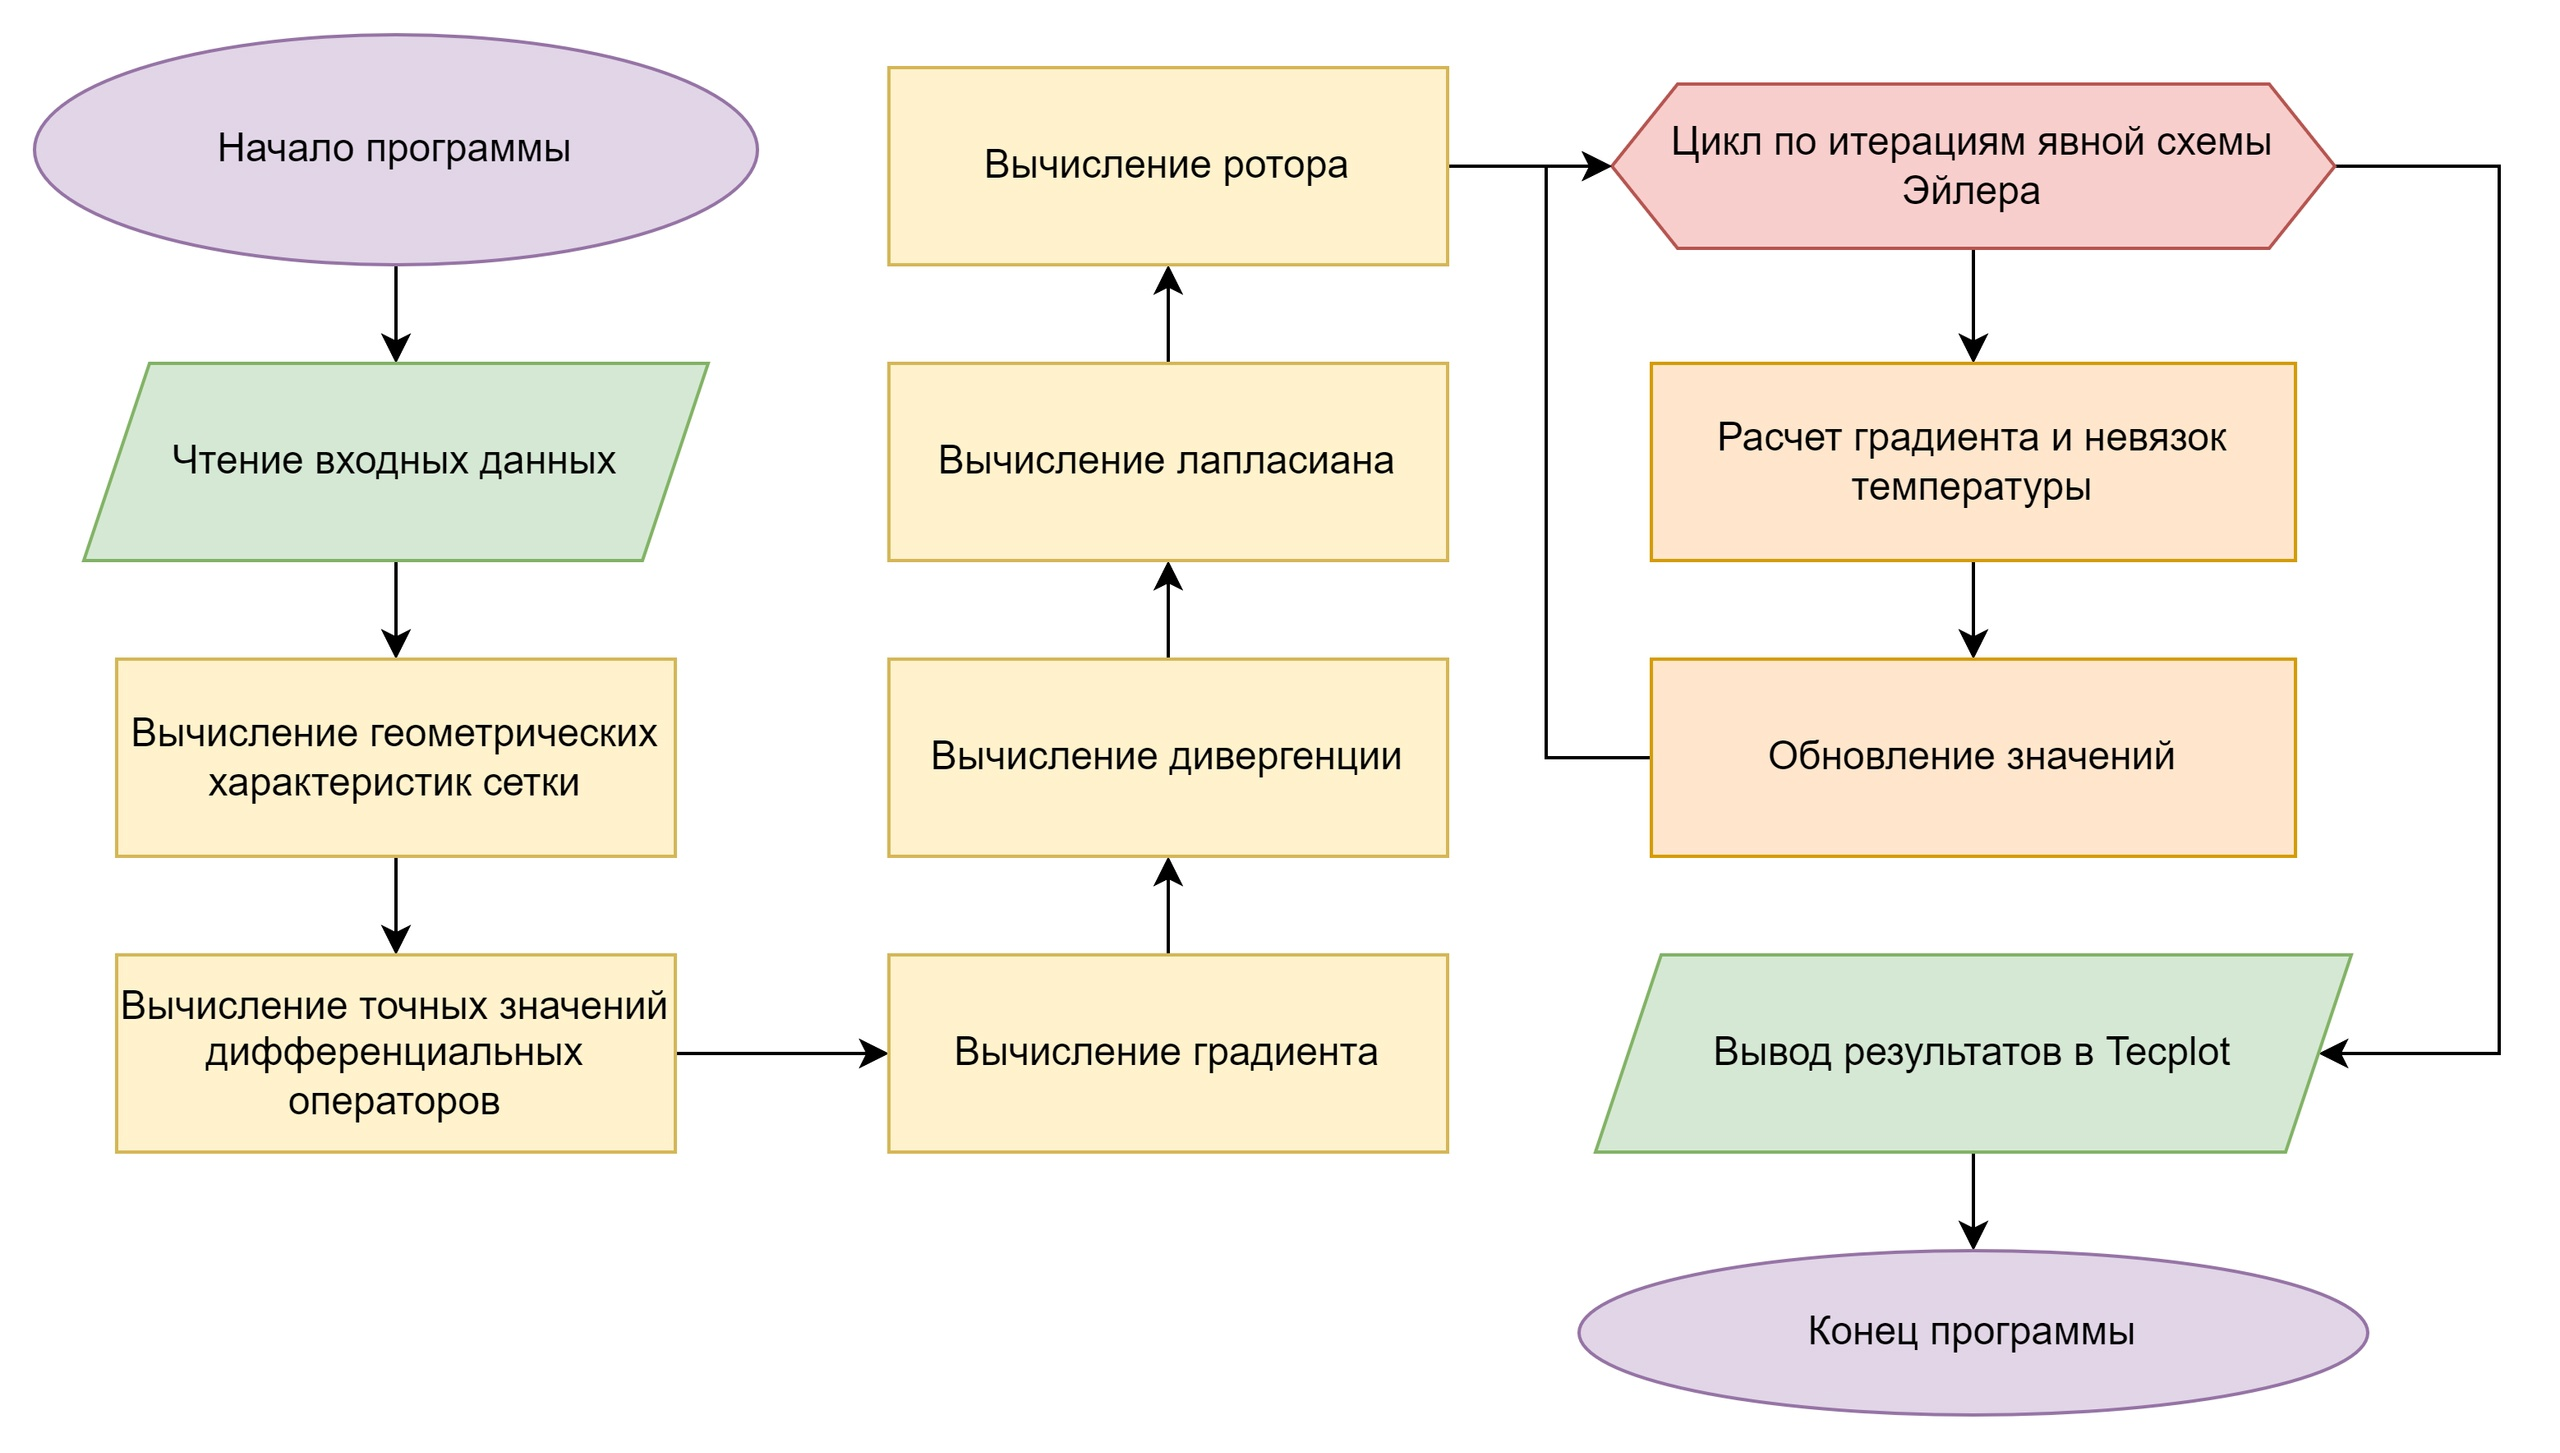
\includegraphics[width=0.55\textwidth]{img/9.jpg}
    \caption{Блок схема вычислительной программы.}
    \label{fig:9}
\end{figure}

Для структурирования кода программа была реализована в модульном варианте. Далее будет описана работа каждого из модулей:

{1. Модуль A\_Main.f90}
Данный модуль является управляющим и основным. В нём производится чтение входного файла \texttt{input.txt}, который содержит следующие параметры:
\begin{enumerate}
    \item Имя файла, содержащего необходимую расчетную сетку;
    \item Номер метода расчета градиента давления $\nabla \phi$;
    \item Номер схемы расчета скалярной величины при вычислении $\nabla \cdot (\phi \mathbf{V})$;
    \item Номер схемы расчета конвективных потоков при решении уравнения переноса температуры $T$;
    \item Масштаб скорости $V$;
    \item Масштаб длины $L$;
    \item Число Рейнольдса $Re$;
    \item Число Прандтля $Pr$;
    \item Число Куранта $CFL$;
    \item Число фон Неймана $VNM$;
    \item Количество итераций при решении уравнения переноса $T$;
\end{enumerate}

Далее производится чтение количества узлов расчетной сетки $N_I$, $N_J$, выделение памяти под массивы и чтение самих узлов расчетной сетки из файла, указанного в \texttt{input.txt}. После этого, если решается задача о течении в каверне, заполняются массивы полей $T_{flos}$ и $\mathbf{V}_{flos}$, полученные в ходе расчета в программе Flos. Следующим этапом является расчет геометрических характеристик, который выполняется в модуле \texttt{B\_CalcMetric.f90}.

После инициализации полей $p$ и $\mathbf{V}$ производится расчет точных значений дифференциальных операторов, поочередное вычисление пространственных дифференциальных операторов и вывод в консоль максимальных значений погрешности. Затем решается уравнение переноса $T$, а результаты записываются в файл с использованием модуля \texttt{B\_OutputFields.f90}.

{2. Модуль B\_CalcMetric.f90}
Этот модуль используется для вычисления геометрических характеристик расчетной сетки. В нём для каждой ячейки вычисляются:
\begin{itemize}
    \item центры граней $\mathbf{r}_f$;
    \item векторы нормали к грани $\mathbf{I}_n$ или $\mathbf{J}_n$ в зависимости от направления (индекса $i$ или $j$);
    \item объём каждой ячейки $\Omega$;
    \item центр ячейки $\mathbf{r}_c$, с учётом особенностей приграничных ячеек.
\end{itemize}

{3. Модуль B\_Functions.f90}
Этот модуль содержит функции для:
\begin{itemize}
    \item вычисления полей $p$ и $\mathbf{V}$;
    \item расчета точных значений пространственных дифференциальных операторов в виде полиномиальных функций от $x$ и $y$;
    \item вычисления значения переменной по методу линейной интерполяции.
\end{itemize}

{4. Модуль B\_CalcGradient.f90}
Модуль предназначен для численного расчета градиента скалярной функции $\nabla \phi$ методами Грина-Гаусса и Грина-Гаусса с итерациями. Для каждой грани определяются:
\begin{itemize}
    \item значение $\phi_f$;
    \item вектор площади грани $\sigma_f$;
    \item центр грани $\mathbf{r}_f$;
    \item индексы соседних ячеек.
\end{itemize}

{5. Модуль B\_CalcDivergence.f90}
В этом модуле реализован численный расчет дивергенции произведения $\phi \cdot \mathbf{V}$ с использованием схем \texttt{Central}, \texttt{FOU}, \texttt{SOU}.

{6. Модуль B\_CalcLapl.f90}
Реализован численный расчет лапласиана скалярной величины $\phi$. Инициализируется массив для лапласиана, а затем вычисляются вектор площади грани $\sigma_f$, центр грани $\mathbf{r}_f$ и индексы соседних ячеек.

{7. Модуль B\_CalcRotor.f90}
Модуль отвечает за численный расчет ротора векторного поля $\mathbf{V}$. Инициализация массива и определение геометрических характеристик проводятся аналогично другим модулям.

{8. Модуль B\_OutputFields.f90}
Результаты расчетов записываются в файлы с расширением \texttt{.plt} для последующей обработки в \texttt{Tecplot}.

{Решение уравнения конвективно-диффузионного переноса температуры}
Решение задачи о течении в каверне с движущейся крышкой осуществляется итерационно. Инициализируются поле температуры $T_1 = 1$ и граничные условия:
\begin{itemize}
    \item $T = 1$ на левой стенке ($i = 0$ и $j = 1, N_J - 1$);
    \item $T = 2$ на правой стенке ($i = N_I$ и $j = 1, N_J - 1$).
\end{itemize}
В модуле \texttt{B\_CalcResT.f90} рассчитываются невязки $Res_T$ и значения температуры обновляются на каждой итерации.

{Параллельные вычисления}
Для исследования эффективности распараллеливания процесса использовались конструкции из пакета OpenMP:
\begin{itemize}
    \item \texttt{OMP DO} для автоматического распределения итераций цикла между потоками;
    \item \texttt{private()} для определения локальных копий переменных;
    \item \texttt{single} для выполнения блока кода одной нитью.
\end{itemize}

Время работы параллельной области определялось с помощью функции \texttt{OMP\_GET\_WTIME()}, а число потоков задавалось переменной окружения \texttt{OMP\_NUM\_THREADS}.


\section{Результаты исследований реализованных методов расчета пространственных дифференциальных операторов.}

на рисунке \ref{fig:10} представлены три различных расчетные сетки, используемые при вычислении пространственных операторов и отладки программы. Расчетная область представляет собой квадрат. Базовая и скошенная расчетная сетка имеет размеры 21 на 21 узел, имельченная 61 на 61.

\begin{figure}
    \centering
    \subcaptionbox{Base mesh}{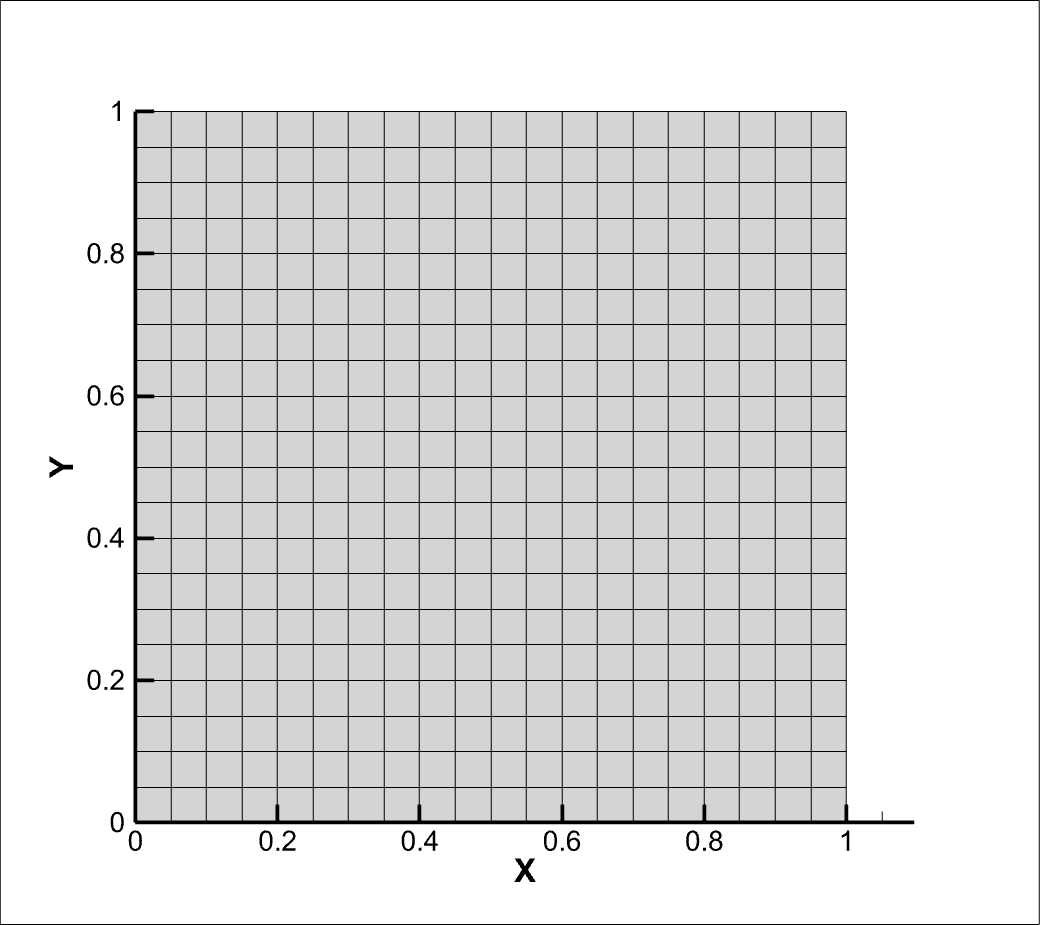
\includegraphics[width=0.3\textwidth]{img/10.1.png}}
    \subcaptionbox{Skew mesh}{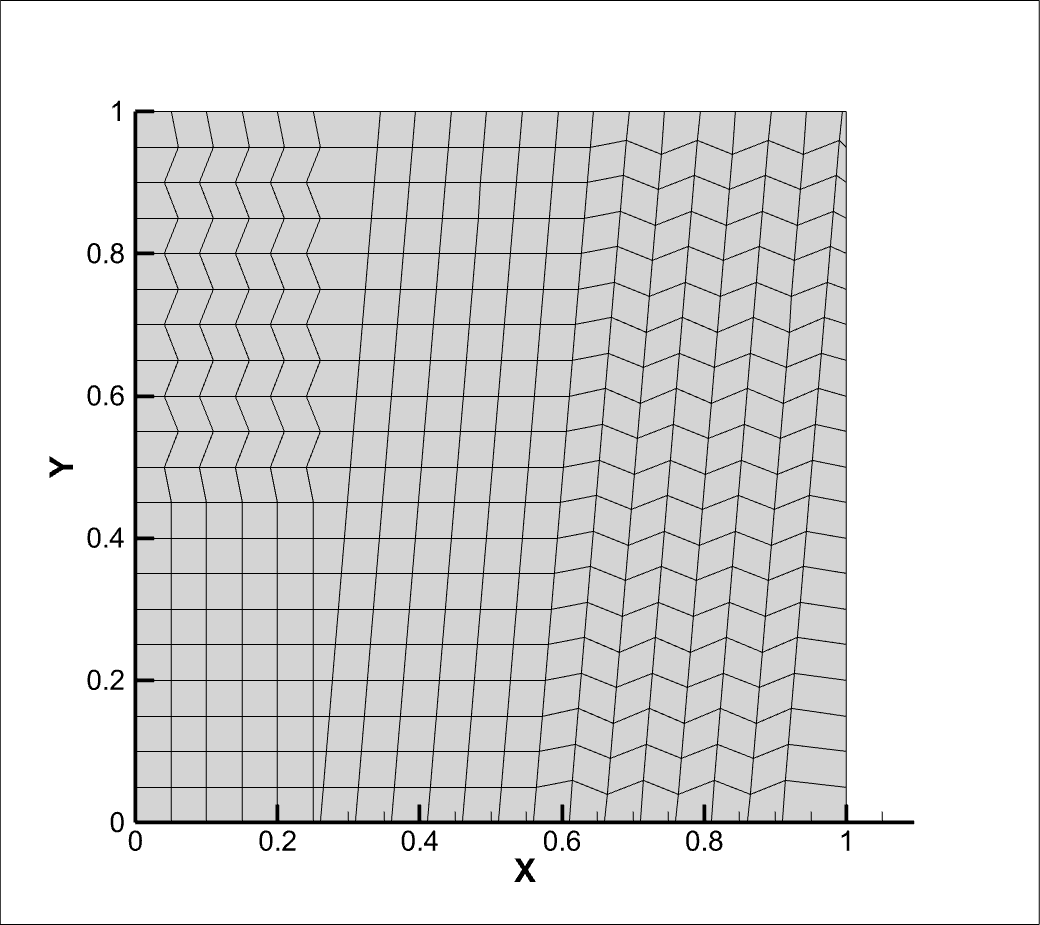
\includegraphics[width=0.3\textwidth]{img/10.2.png}}
    \subcaptionbox{Fine mesh}{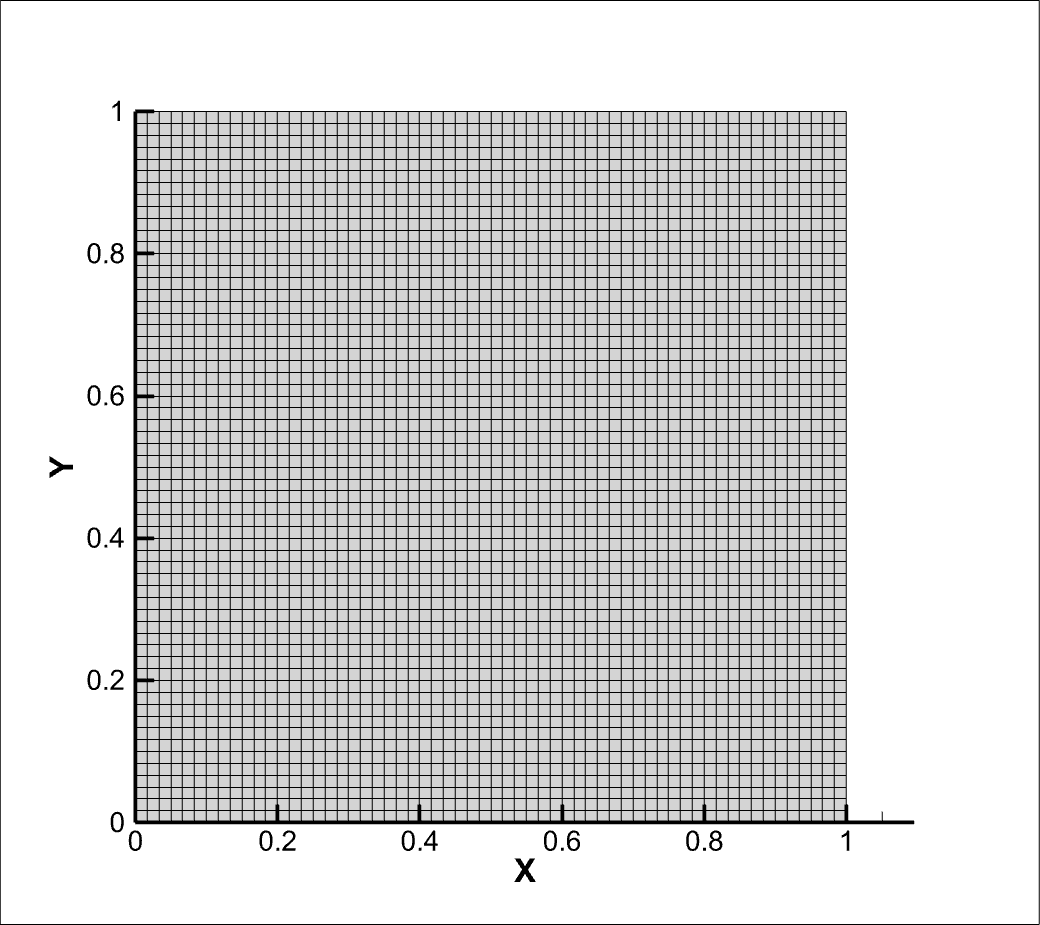
\includegraphics[width=0.3\textwidth]{img/10.3.png}}
    \caption{Различные виды сеток.}
    \label{fig:10}
\end{figure}

При вычислении дифференциальных операторов вычислялась точность расчета с помощью относительной ошибки:

$$Error(...) = |\frac{(...)_{ex}-(...)_{num}}{(...)_{ex}}|,$$
где $(...)_{ex}$ - точное значение дифференицального оператора, $(...)_{num}$ - численное значение дифф. оператора.

Для определения порядка точности производились расчет при одинх и тех же паратрах на базовой сетке и измельченной, определялись ошибки и после порядок находился по формуле:

\begin{equation}
    O(...) = log_\frac{h_{b}}{h_{f}} (\frac{Error(...)_{base}}{Error(...)_{fine}})
\end{equation}

Для проведения расчетов использовался первый порядок точности так как погрешности этих методов и схем значительно превышают порядок машинной погрешности.


В таблице \ref{tab:1} представлены полиномы различных степеней для скалярного поля p, а также соответствующие им значения скалярных операторов. При расчете дивергенции необходимо использовать векторное поле, поэтому было определено оно равным: $\vec{V} = (1,1)$.


\begin{table}[H]
    \centering
    \caption{Виды полиномов используемых в дальнеших расчетах с точными операторами}
    \resizebox{\textwidth}{!}{%
    \begin{tabular}{|l|c|c|c|c|l|}
    \hline
       & $p$               & $\nabla p_x$ & $\nabla p_y$ & $\nabla\cdot(p\vec{V})$ & $\Delta p$ \\ \hline
    P1 & $x+3y$            & 1            & 3            & 4                       & 0          \\ \hline
    P2 & $x^2+y^2+2xy+x+y$ & $1+2x+2y$    & $1+2x+2y$    & $2+4x+4y$               & 4          \\ \hline
    P3 &
      \multicolumn{1}{l|}{$x^3+5y^3+x^2y+y^2x+xy+x+y$} &
      \multicolumn{1}{l|}{$1+3x^2+y+y^2+2xy$} &
      \multicolumn{1}{l|}{$1+x+x^2+2xy+15y^2$} &
      \multicolumn{1}{l|}{$2+x+4x^2+y+4xy+16y^2$} &
      $8(x+4y)$ \\ \hline
    P4 & $x^4+y^4+x^2+y^2 $ & $4x^3+2x$ & $4y^3+2y$&$4x^3+4y^3+2x+2y$&$12(x^2+y^2)+4$ \\
      
      
      \hline

    \end{tabular}%
    }
    
    \label{tab:1}
\end{table}


В таблице \ref{tab:2} представлены полиномы различных степеней для компонент векторного поля, а также соответствующие им значения z-компоненты оператора ротора.

% Please add the following required packages to your document preamble:
% \usepackage{graphicx}
\begin{table}[H]
    \centering
    \caption{Виды полиномов используемых в дальнеших расчетах с точным ротором векторного поля}
    \resizebox{\textwidth}{!}{%
    \begin{tabular}{|l|c|c|c|}
    \hline
       & $u$         & $v$        & $rot\vec{V}_z$ \\ \hline
    P1 & $y$         & $-3x$      & -4             \\ \hline
    P2 & $y^2-4xy+y$ & $x^2+xy+x$ & $6x-y$         \\ \hline
    P3 & \multicolumn{1}{l|}{$-3y^3-xy-y$} & \multicolumn{1}{l|}{$x^3-xy+4x$} & \multicolumn{1}{l|}{$3x^2+9y^2+x-y+5$} \\ \hline
    \end{tabular}%
    }

    \label{tab:2}
\end{table}

\subsection{Расчет градиента скалярного поля.}
Для расчета градиента скалярного поля были использованы методы Грина-Гаусса и метод Грина-Гаусса с итерациями. В результате расчетов были определены максимальные среди двух компонент градиента ошибки наибольшие для всех ячеек. При расчетах на базовой и измельченной расчетных сетках также определялась ошибка в центре расчетной области. Полученные значение представлены в таблице \ref{tab:3}.


\begin{table}[H]
    \centering
    \resizebox{\textwidth}{!}{%
    \begin{tabular}{|cc|cc|cc|}
    \hline
    \multicolumn{2}{|c|}{} &
      \multicolumn{2}{c|}{Без итераций} &
      \multicolumn{2}{c|}{С итерациями} \\ \hline
    \multicolumn{1}{|c|}{Вид сетки} &
      P &
      \multicolumn{1}{c|}{max(Error)} &
      Error в центре &
      \multicolumn{1}{c|}{max(Error)} &
      Error в центре \\ \hline
    \multicolumn{1}{|c|}{} &
      P1 &
      \multicolumn{1}{c|}{1.32e-5} &
      3.66e-6 &
      \multicolumn{1}{c|}{1.31e-5} &
      3.65e-6 \\ \cline{2-6} 
    \multicolumn{1}{|c|}{} &
      P2 &
      \multicolumn{1}{c|}{4.26e-6} &
      6e-7 &
      \multicolumn{1}{c|}{1.13e-2} &
      8e-7 \\ \cline{2-6} 
    \multicolumn{1}{|c|}{\multirow{-3}{*}{Base}} &
      P3 &
      \multicolumn{1}{c|}{1.2e-2} &
      8e-4 &
      \multicolumn{1}{c|}{1.23e-2} &
      7.9e-4 \\ \hline
    \multicolumn{1}{|c|}{Fine} &
      P3 &
      \multicolumn{1}{c|}{1.37e-3} &
      8.96e-5 &
      \multicolumn{1}{c|}{3.87e-3} &
      9.19e-5 \\ \hline
    \multicolumn{1}{|c|}{} &
      P1 &
      \multicolumn{1}{c|}{1.69} &
      \cellcolor[HTML]{9B9B9B} &
      \multicolumn{1}{c|}{2.98e-5} &
      \cellcolor[HTML]{9B9B9B} \\ \cline{2-6} 
    \multicolumn{1}{|c|}{\multirow{-2}{*}{Skew}} & P2 & \multicolumn{1}{c|}{0.65} & \cellcolor[HTML]{9B9B9B} & \multicolumn{1}{c|}{1.13e-2} & \cellcolor[HTML]{9B9B9B} \\ \hline
    \end{tabular}%
    }
    \caption{Ошибка вычислений для различных вариантов}
    \label{tab:3}
\end{table}


Оценим порядок точности для полинома третье степени. Получим, что для метода Грина Гаусса порядок точности для приграничных и внутренних ячеек соответственно равен:

$$O(\nabla p)_b = 1.975$$
$$O(\nabla p)_{inner} = 1.993$$

Для метода Грина Гаусса с итерациями соответственно:

$$O(\nabla p)_b = 1.053$$
$$O(\nabla p)_{inner} = 1.95$$

Видно, что для метода Грина-Гаусса с итерациями имеем первый порядок точности для пограничных ячеек, потому что в нем не вводили поправку второго порядка для приграничных ячеек.

На рисунках \ref{fig:11} - \ref{fig:16} представлены x-компоненты градиента скаляра при расчете на разных сетках с разным полиномом. Посколько для другой компоненты ситуация аналогичная оставим только эту. 

\begin{figure}[H]
    \centering
    \subcaptionbox{GG}{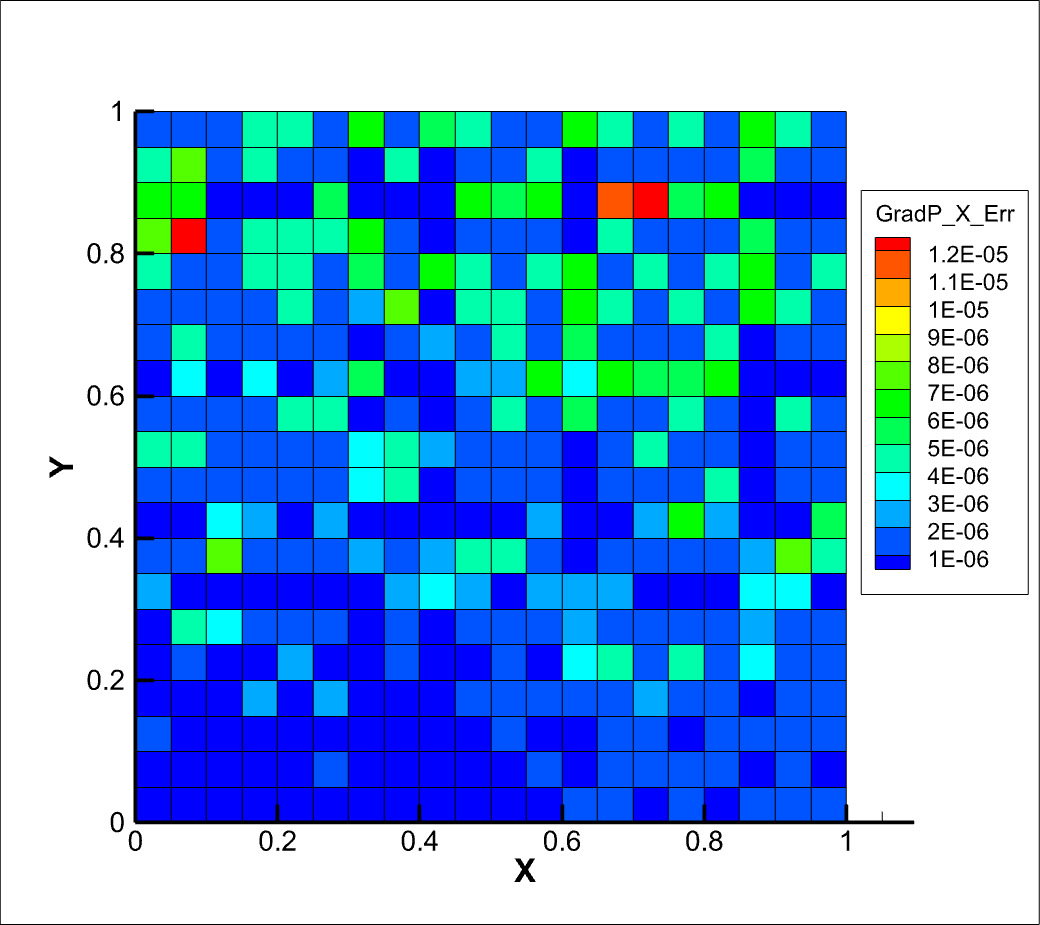
\includegraphics[width=0.45\textwidth]{img/11.1.png}}
    \subcaptionbox{GG with iteration}{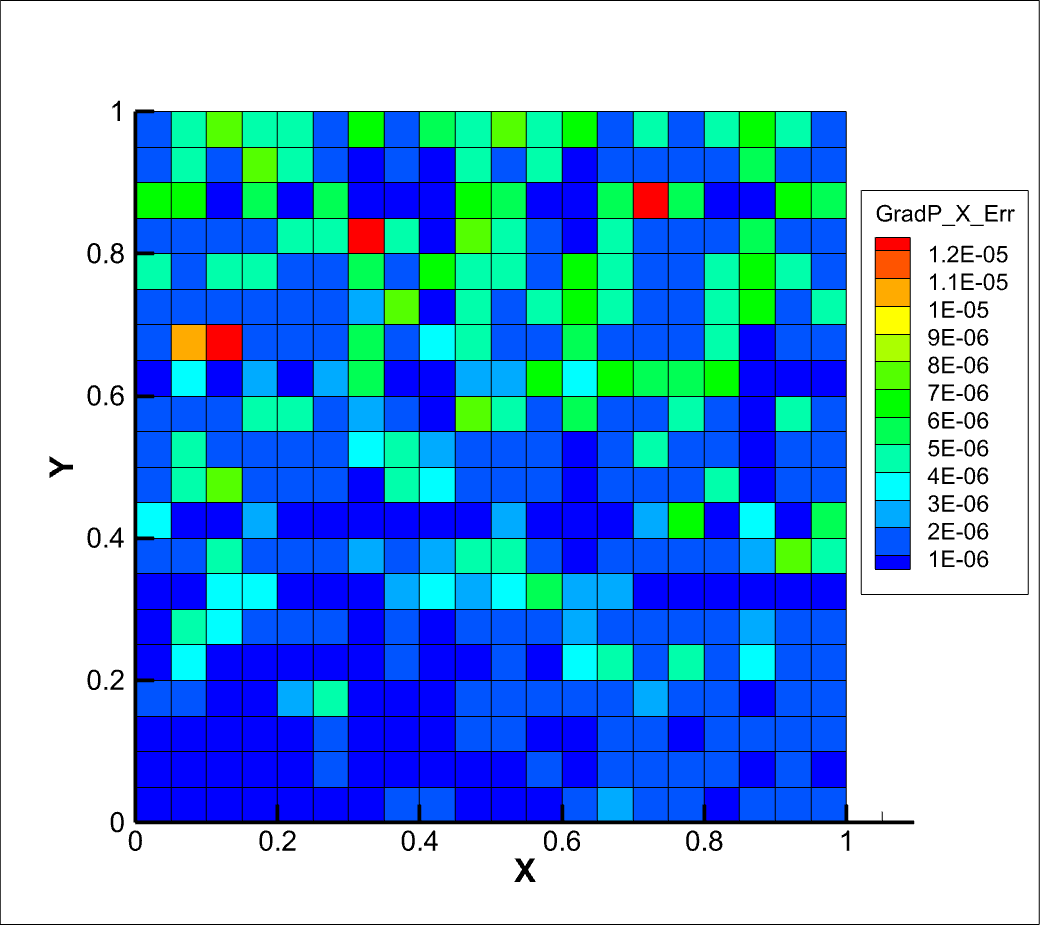
\includegraphics[width=0.45\textwidth]{img/11.2.png}}
    \caption{Распределение ошибки для полинома первой степени на base сетке.}
    \label{fig:11}
\end{figure}

\begin{figure}[H]
    \centering
    \subcaptionbox{GG}{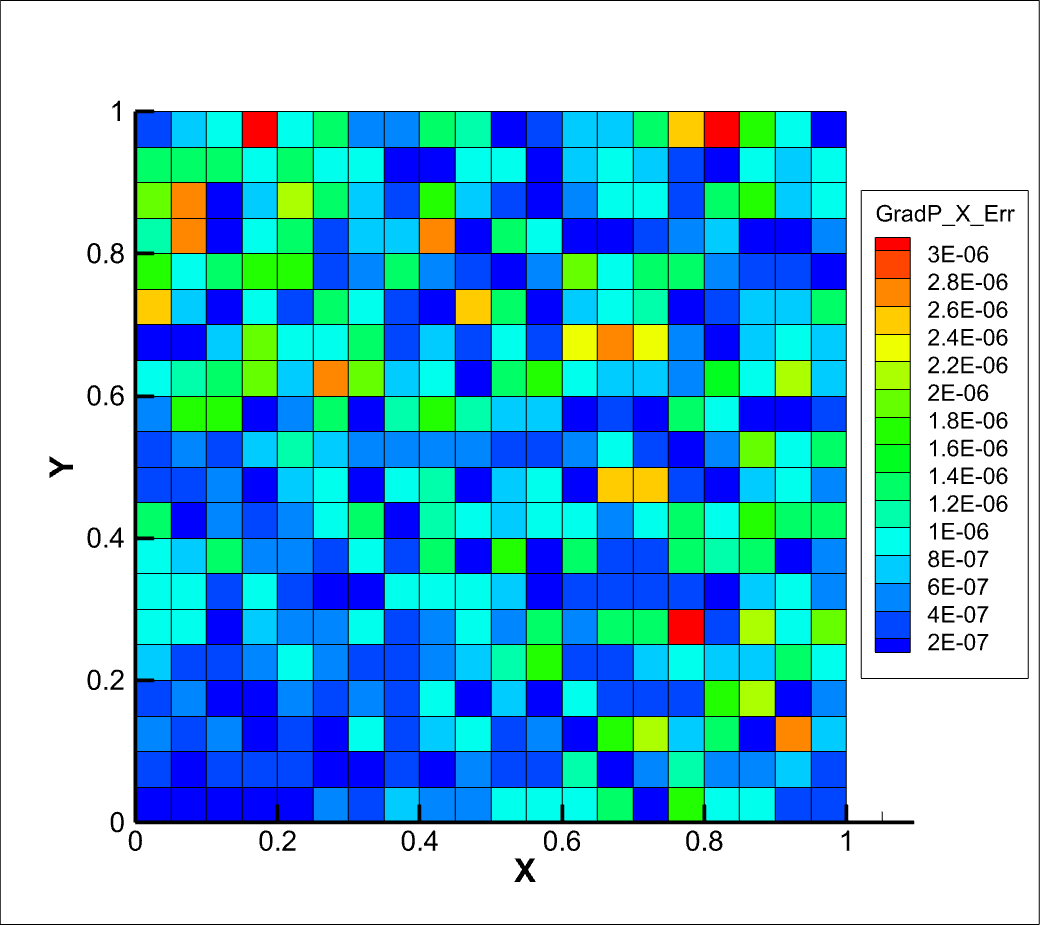
\includegraphics[width=0.45\textwidth]{img/12.1.png}}
    \subcaptionbox{GG with iteration}{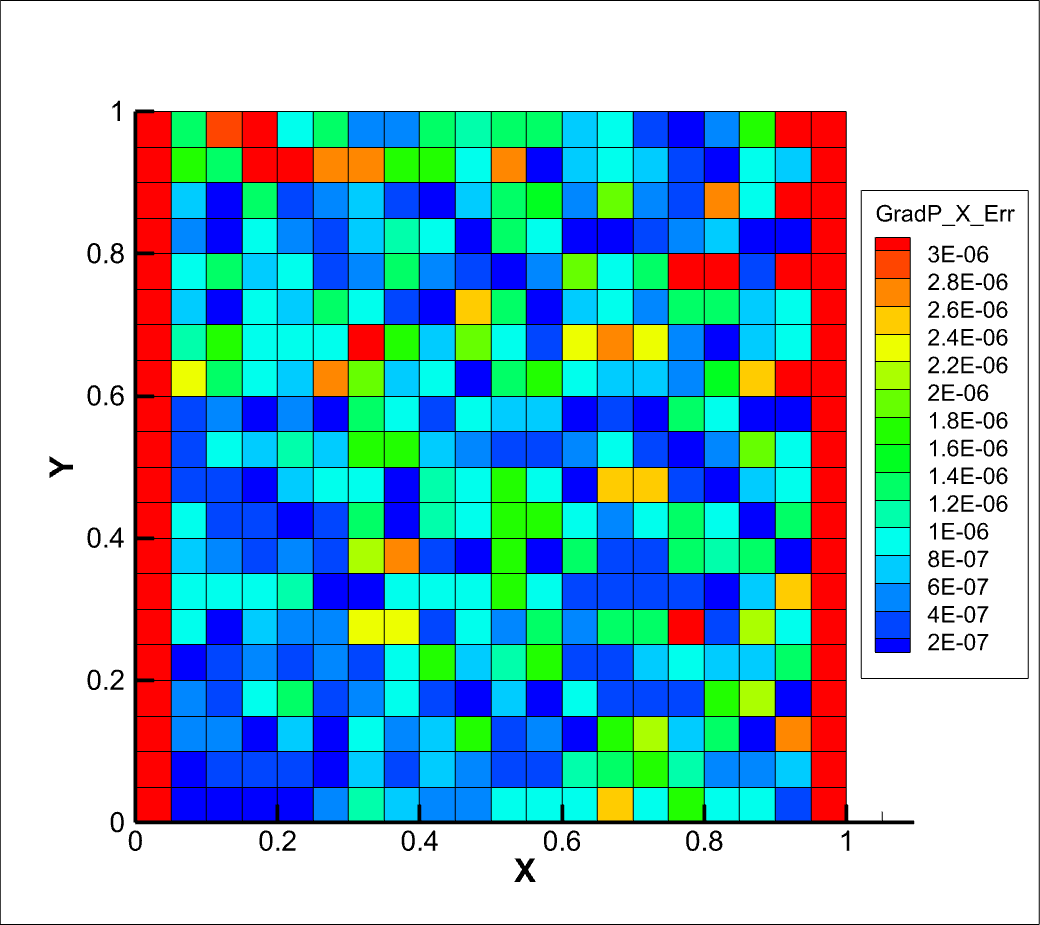
\includegraphics[width=0.45\textwidth]{img/12.2.png}}
    \caption{Распределение ошибки для полинома второй степени на base сетке.}
    \label{fig:12}
\end{figure}


\begin{figure}[H]
    \centering
    \subcaptionbox{GG}{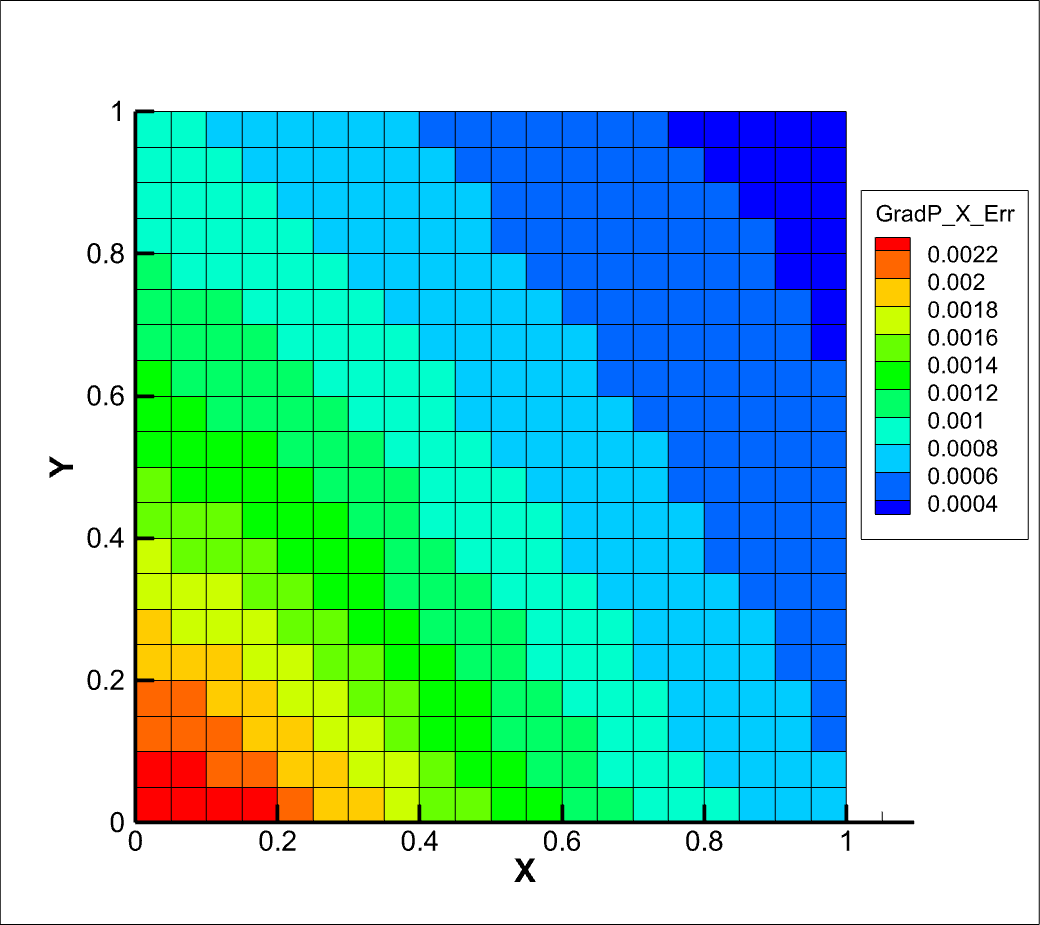
\includegraphics[width=0.45\textwidth]{img/13.1.png}}
    \subcaptionbox{GG with iteration}{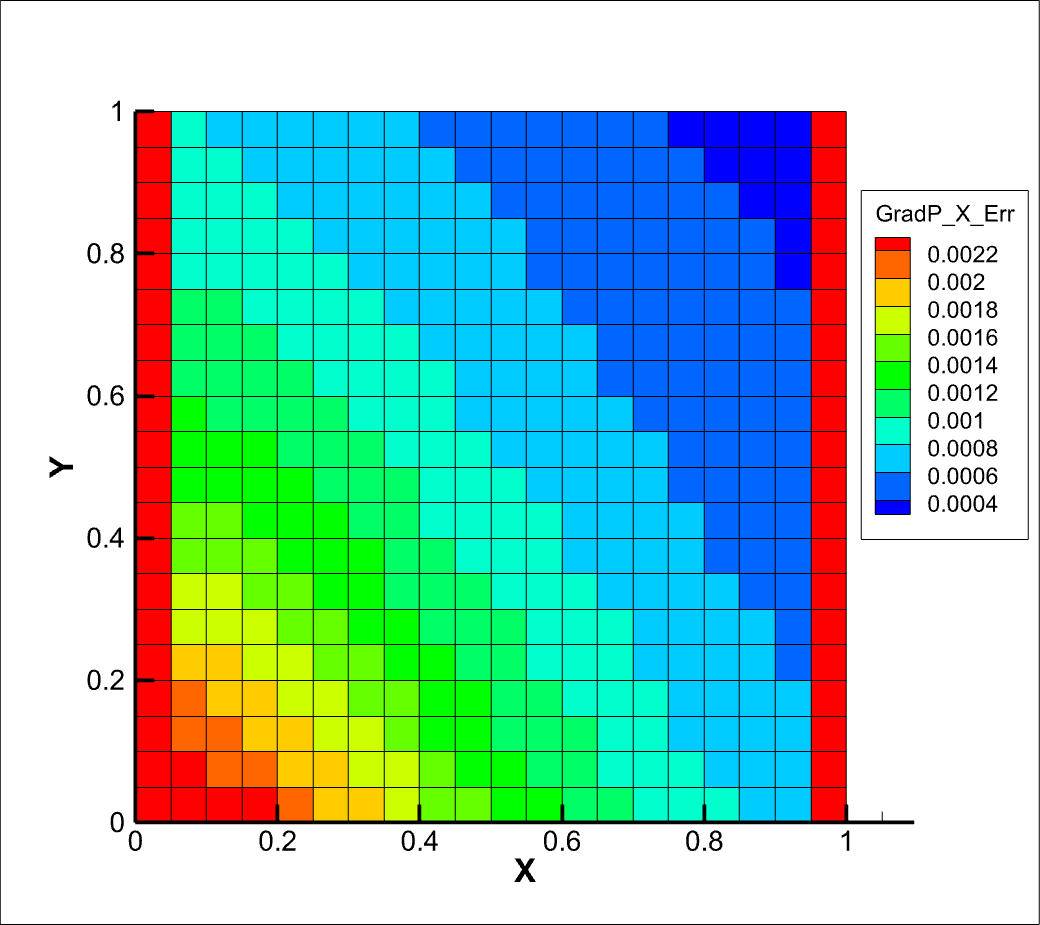
\includegraphics[width=0.45\textwidth]{img/13.2.png}}
    \caption{Распределение ошибки для полинома третьей степени на base сетке.}
    \label{fig:13}
\end{figure}

\begin{figure}[H]
    \centering
    \subcaptionbox{GG}{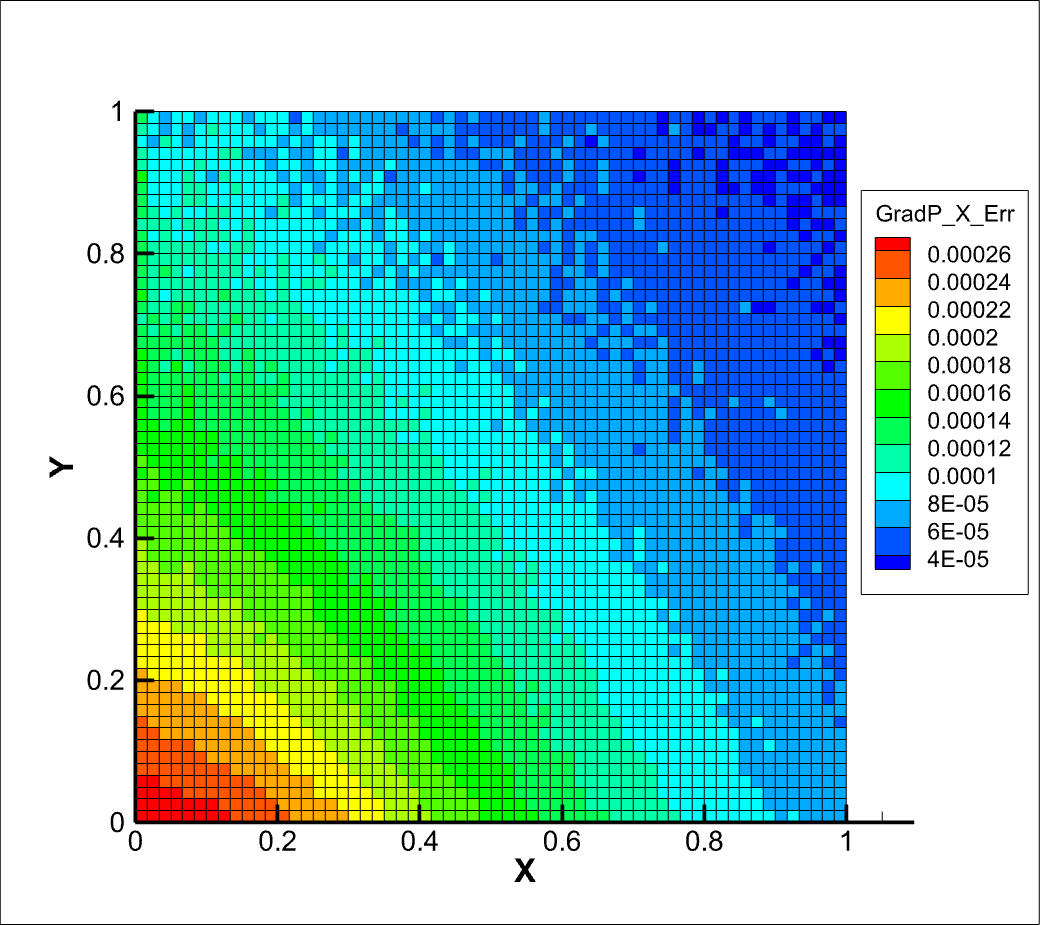
\includegraphics[width=0.45\textwidth]{img/14.1.png}}
    \subcaptionbox{GG with iteration}{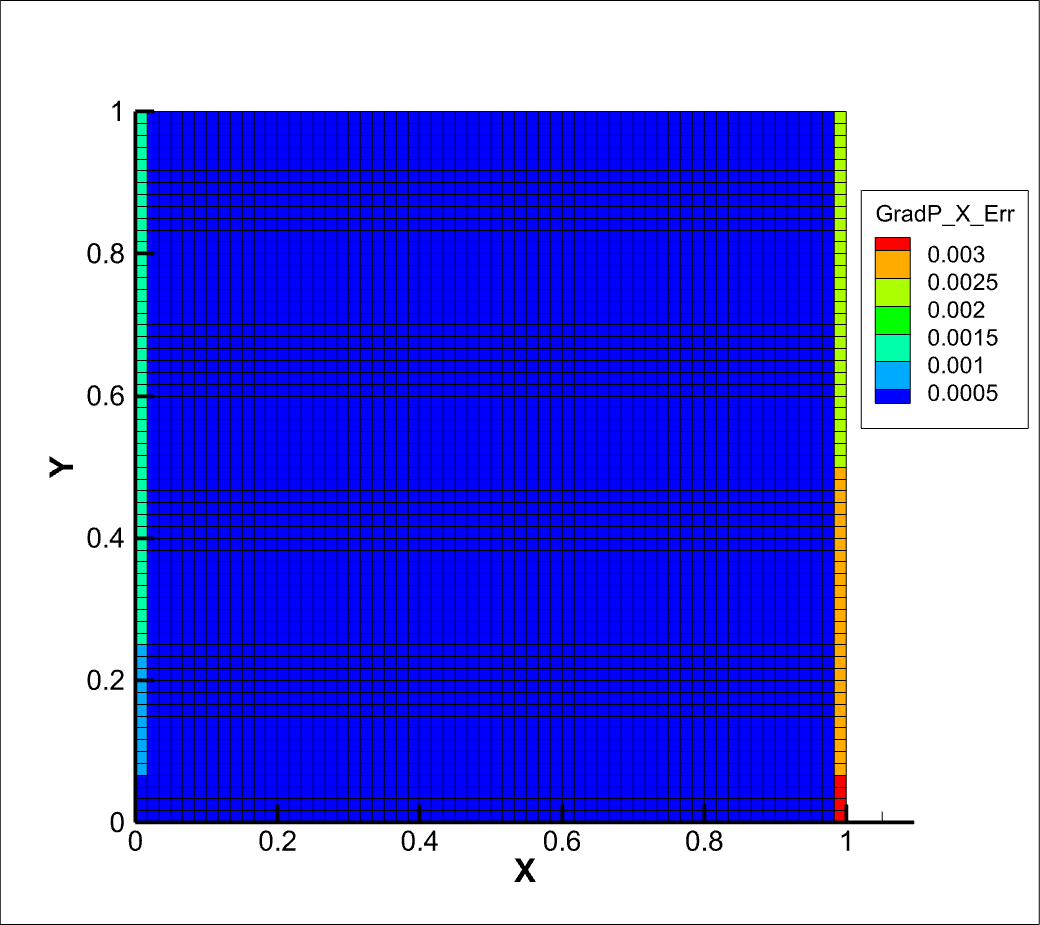
\includegraphics[width=0.45\textwidth]{img/14.2.png}}
    \caption{Распределение ошибки для полинома третьей степени на fine сетке.}
    \label{fig:13}
\end{figure}

\begin{figure}[H]
    \centering
    \subcaptionbox{GG}{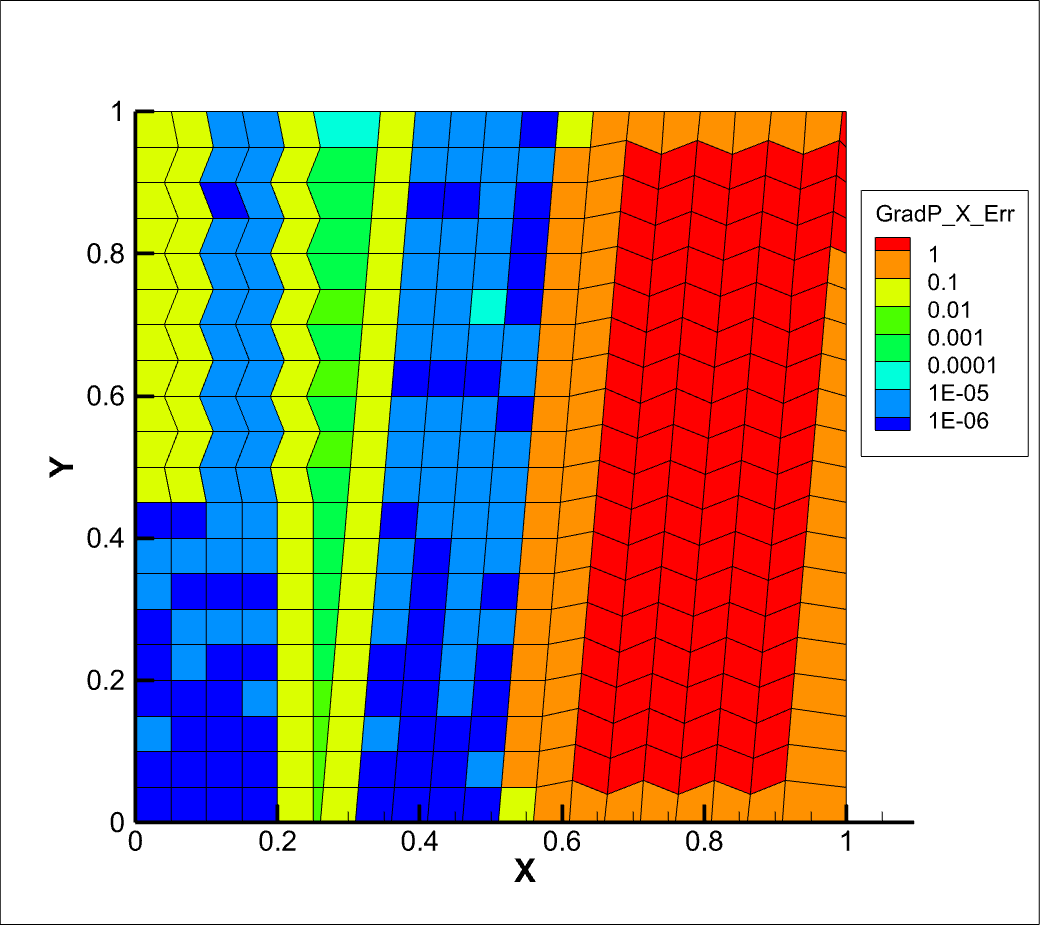
\includegraphics[width=0.45\textwidth]{img/15.1.png}}
    \subcaptionbox{GG with iteration}{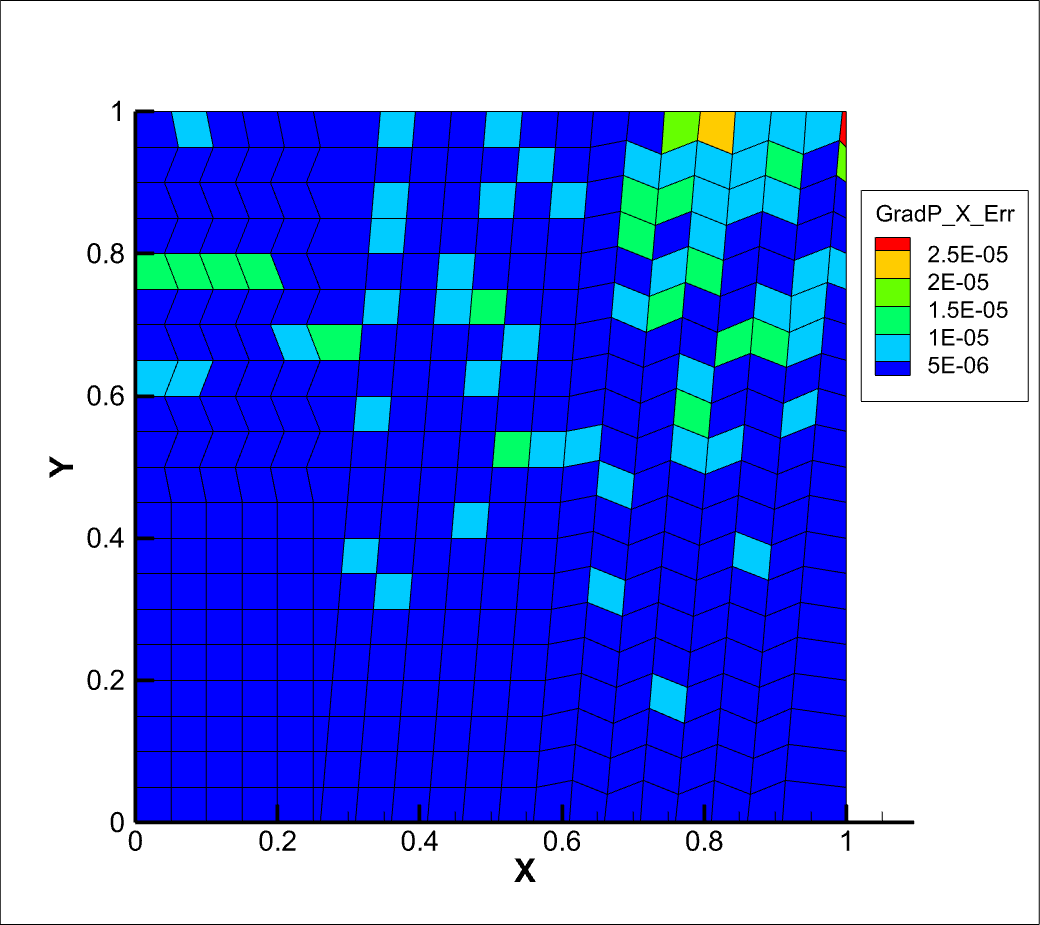
\includegraphics[width=0.45\textwidth]{img/15.2.png}}
    \caption{Распределение ошибки для полинома первой степени на base сетке.}
    \label{fig:15}
\end{figure}

\begin{figure}[H]
    \centering
    \subcaptionbox{GG}{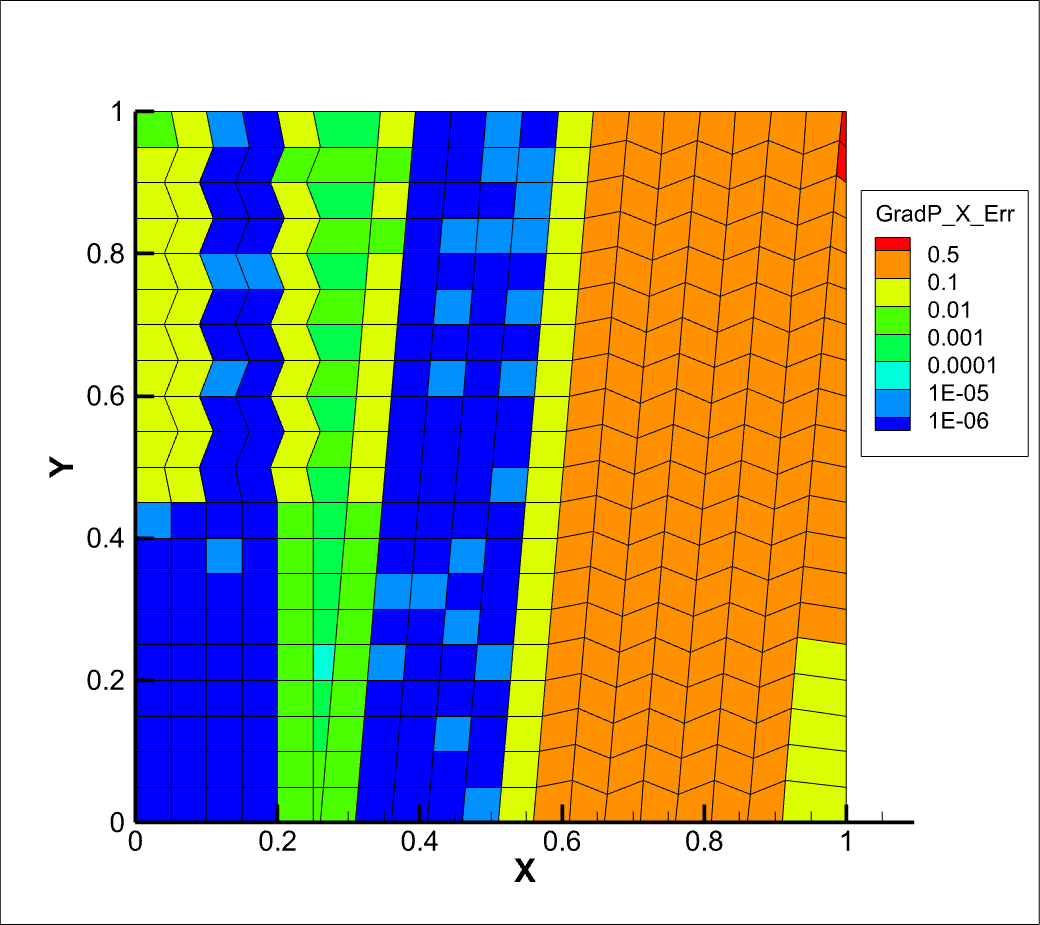
\includegraphics[width=0.45\textwidth]{img/16.1.png}}
    \subcaptionbox{GG with iteration}{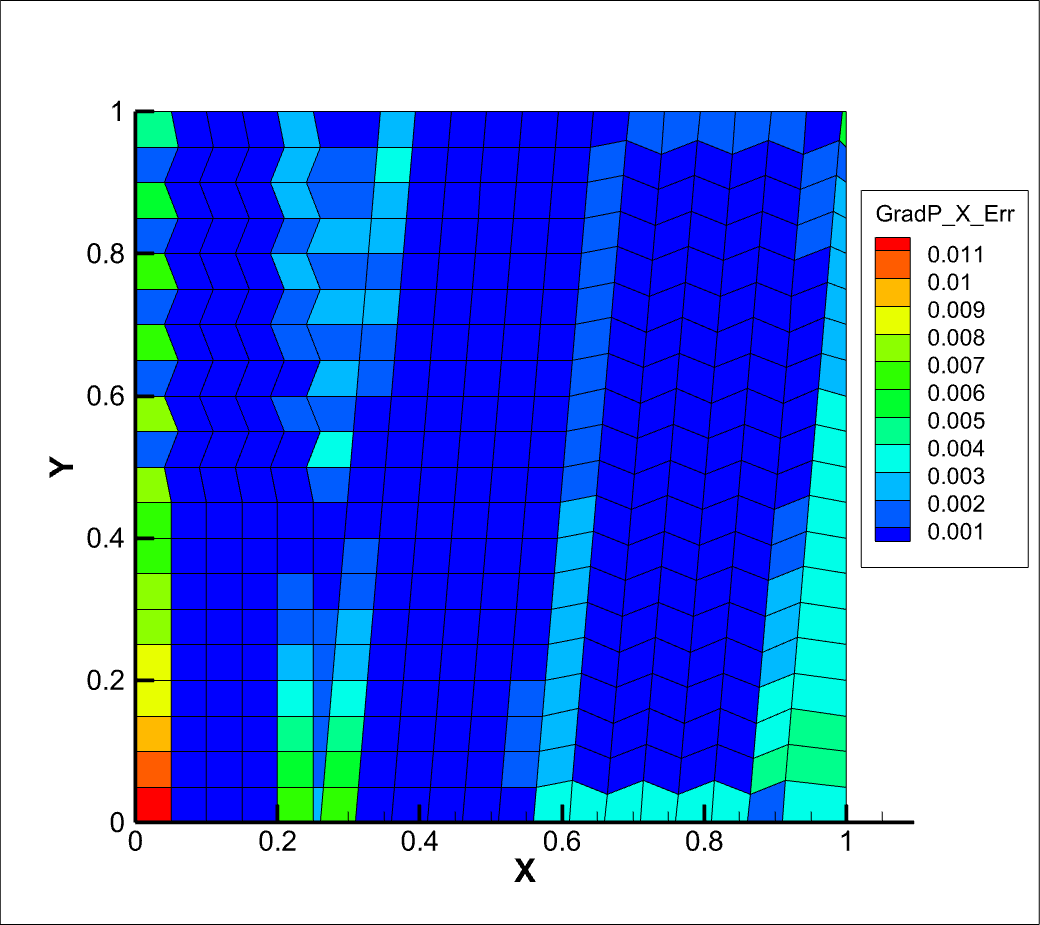
\includegraphics[width=0.45\textwidth]{img/16.2.png}}
    \caption{Распределение ошибки для полинома второй степени на base сетке.}
    \label{fig:16}
\end{figure}

Видно, что для полинома первой степени получаем одинаково точные результаты. В случае полинома второй степени во внутренней области также наблюдается машинная точность, однако для приграничных ячеек присутствуют отличия о которых говорилось ранее. 

При рассмотрении ошибки градиента при расчетах на базовой и измельченной сетках видно, что по тойже причине метод Грина Гаусса с итерациями дает резкое повышение ошибки в пограничных ячейках. Поэтому получили там первый порядок точности, а для внутренних ячеек и там и там второй.


Также на примере рисунков \ref{fig:15} и \ref{fig:16} наблюдаем сильное улучшение расчета градиента при внесении поправки и использовании итерационного метода Грина-Гаусса.

Метод Грина-Гаусса с итерациями для того, чтобы учесть скошенность, предполагает выполнение итераций. Если рассмотреть зависимость точности решения для дввух полиномов на скошенной сетке от количества итераций на рисунке \ref{fig:17}, то видно, что в случае P1 ошибка за 5 итераций падает на 5 порядков, а для P2 ошибка падает только на 2 порядка после 3 итераций и не изменяется. Такое поведение говорит, что поправка на скошенность не влияет на величине максимальной ошибки, вызванной нелинейностью P2, но при этом позволяет снизить ее до уровня сетки base.

\begin{figure}[H]
    \centering
    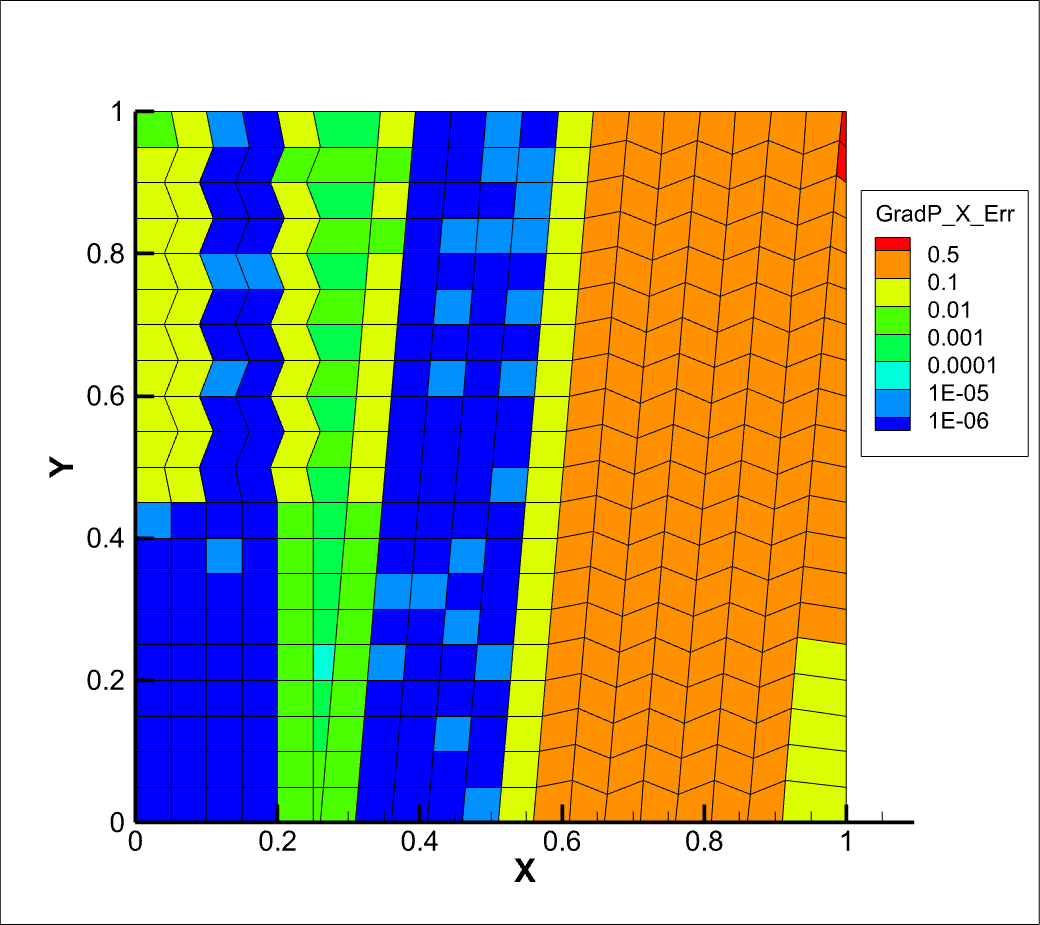
\includegraphics[width=0.45\textwidth]{img/16.1.png}
    \caption{Зависимость ошибки от количества итераций в методе GG с итерациями.}
    \label{fig:17}
\end{figure}

\subsection{Расчет дивергенции произведения скалярной величины на вектор.}

Для расчета дивергенции произведения скалярной величины на вектор были использованы три схемы: FOU, SOU и Central. Использовались полиномы 1-3 степени. Векторно поле было постоянным как и в прошлой задаче. Аналогично предыдущему пункту была построена таблица \ref{tab:4}.


\begin{table}[H]
    \centering
    \caption{Ошибка вычислений для различных вариантов схем интерполяции}
    \resizebox{\textwidth}{!}{%
    \begin{tabular}{|cc|cc|cc|cc|}
    \hline
    \multicolumn{2}{|c|}{}          & \multicolumn{2}{c|}{Central}           & \multicolumn{2}{c|}{FOU}              & \multicolumn{2}{c|}{SOU}               \\ \hline
    \multicolumn{1}{|c|}{Вид сетки} &
      P &
      \multicolumn{1}{c|}{max(Error)} &
      Error в центре &
      \multicolumn{1}{c|}{max(Error)} &
      Error в центре &
      \multicolumn{1}{c|}{max(Error)} &
      Error в центре \\ \hline
    \multicolumn{1}{|c|}{}     & P1 & \multicolumn{1}{c|}{3.63e-6} & 9.17e-7 & \multicolumn{1}{c|}{6.2e-6}  & 7e-7   & \multicolumn{1}{c|}{4.78e-6} & 5.97e-7 \\ \cline{2-8} 
    \multicolumn{1}{|c|}{}     & P2 & \multicolumn{1}{c|}{1.13e-2} & 2.2e-7  & \multicolumn{1}{c|}{3.84e-2} & 1.6e-2 & \multicolumn{1}{c|}{2.72e-2} & 5.5e-7  \\ \cline{2-8} 
    \multicolumn{1}{|c|}{\multirow{-3}{*}{Base}} &
      P3 &
      \multicolumn{1}{c|}{9.3e-3} &
      1.6e-3 &
      \multicolumn{1}{c|}{6.2e-2} &
      5.2e-2 &
      \multicolumn{1}{c|}{1.87e-2} &
      7.5e-4 \\ \hline
    \multicolumn{1}{|c|}{Fine} & P3 & \multicolumn{1}{c|}{3.2e-3}  & 1.7e-4  & \multicolumn{1}{c|}{2.14e-2} & 1.7e-2 & \multicolumn{1}{c|}{2.19e-3} & 8.4e-5  \\ \hline
    \multicolumn{1}{|c|}{Skew} &
      P1 &
      \multicolumn{1}{c|}{0.38} &
      \cellcolor[HTML]{9B9B9B} &
      \multicolumn{1}{c|}{1.81} &
      \cellcolor[HTML]{9B9B9B} &
      \multicolumn{1}{c|}{0.68} &
      \cellcolor[HTML]{9B9B9B} \\ \hline
    \end{tabular}%
    }

    \label{tab:4}
\end{table}

Получили следующие порядки точности для схем:
\begin{itemize}
    \item Central: $O(div(p\vec{V}))_b = 0.97$, $O(div(p\vec{V}))_i = 2.04$
    \item FOU: $O(div(p\vec{V}))_b = 0.96$, $O(div(p\vec{V}))_i = 1.01$
    \item SOU: $O(div(p\vec{V}))_b = 1.95$, $O(div(p\vec{V}))_i = 1.99$
\end{itemize}

На рисункаъ \ref{fig:18} - \ref{fig:22} представлены распределения ошибки для дивергенции для различных схем и сеток.


\begin{figure}[H]
    \centering
    \subcaptionbox{Central}{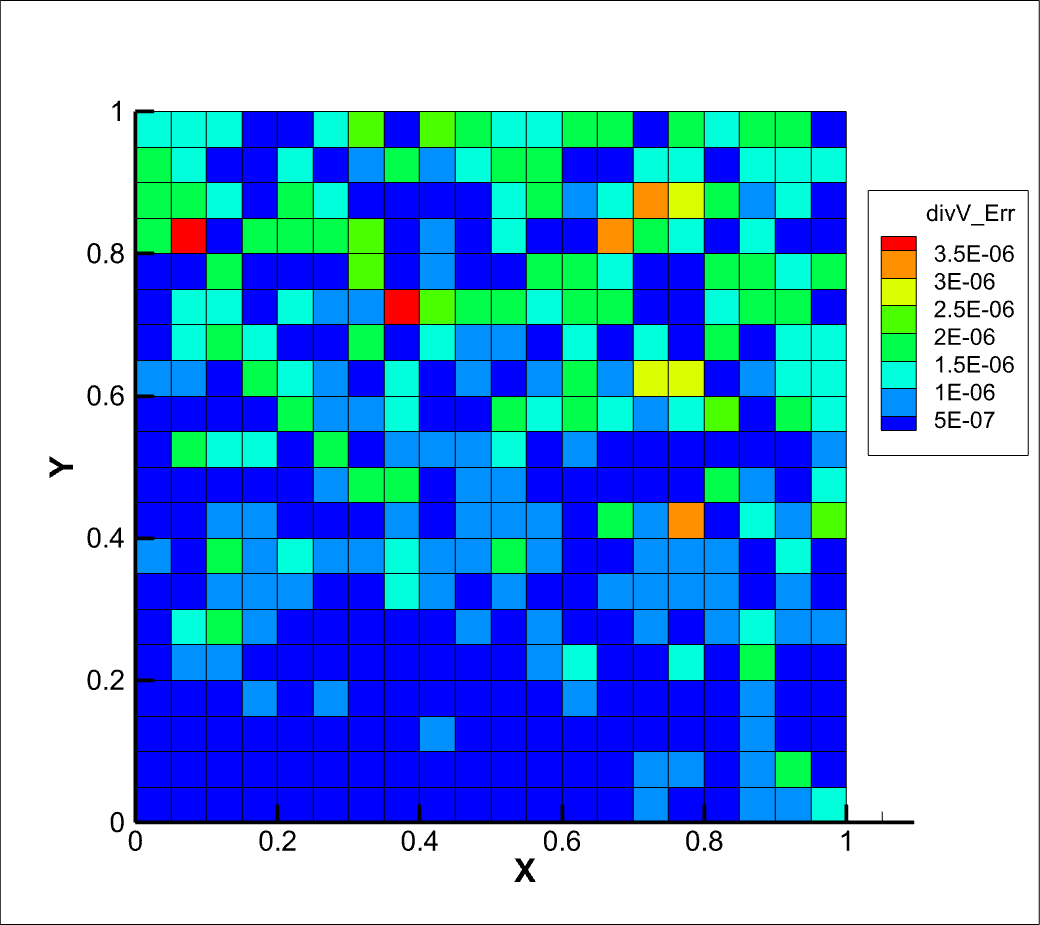
\includegraphics[width=0.3\textwidth]{img/18.1.png}}
    \subcaptionbox{FOU}{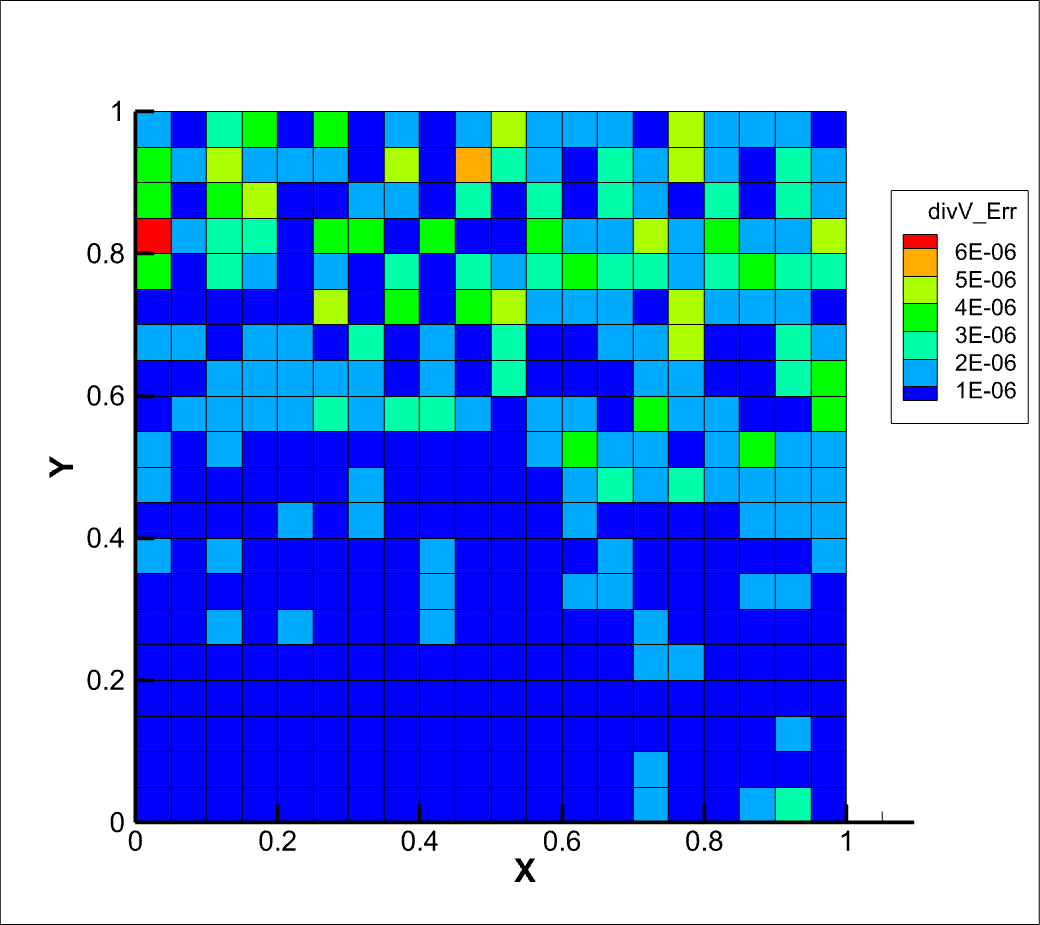
\includegraphics[width=0.3\textwidth]{img/18.2.png}}
    \subcaptionbox{SOU}{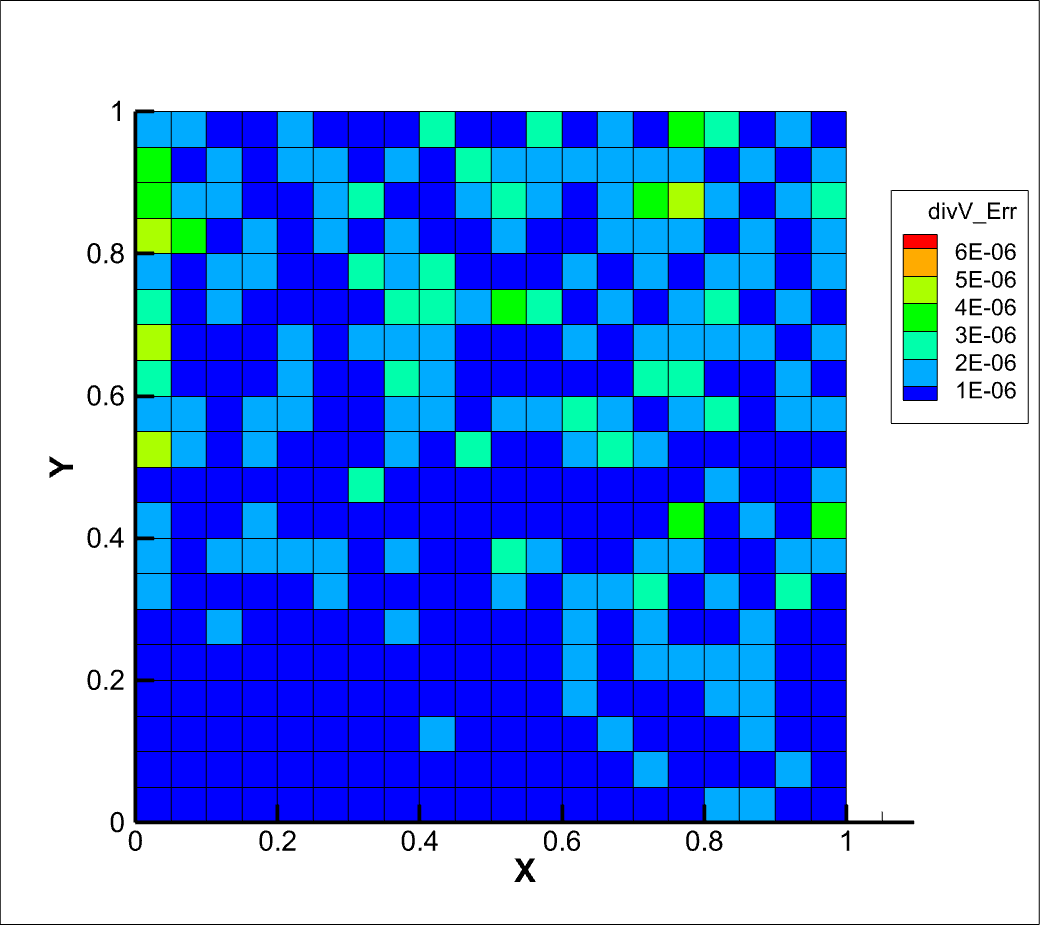
\includegraphics[width=0.3\textwidth]{img/18.3.png}}
    \caption{Распределение ошибки для полинома первой степени на base сетке.}
    \label{fig:18}
\end{figure}

\begin{figure}[H]
    \centering
    \subcaptionbox{Central}{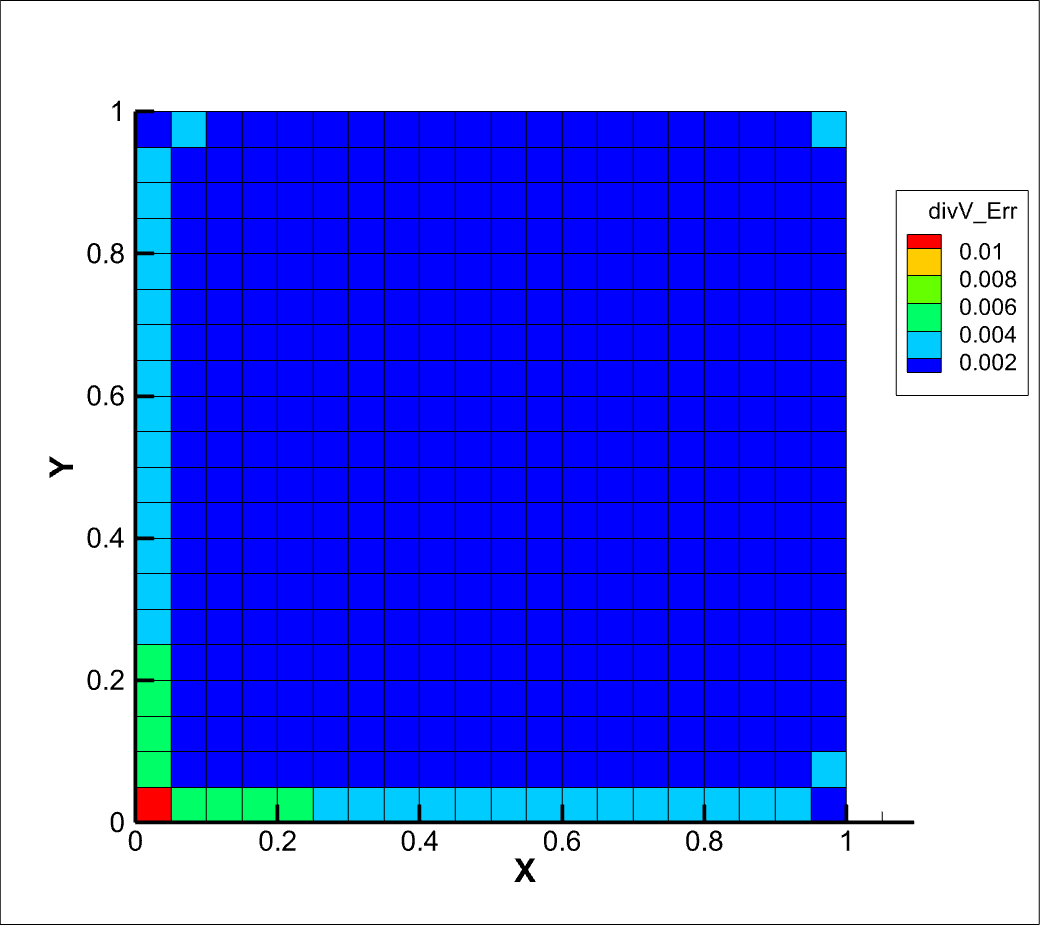
\includegraphics[width=0.3\textwidth]{img/19.1.png}}
    \subcaptionbox{FOU}{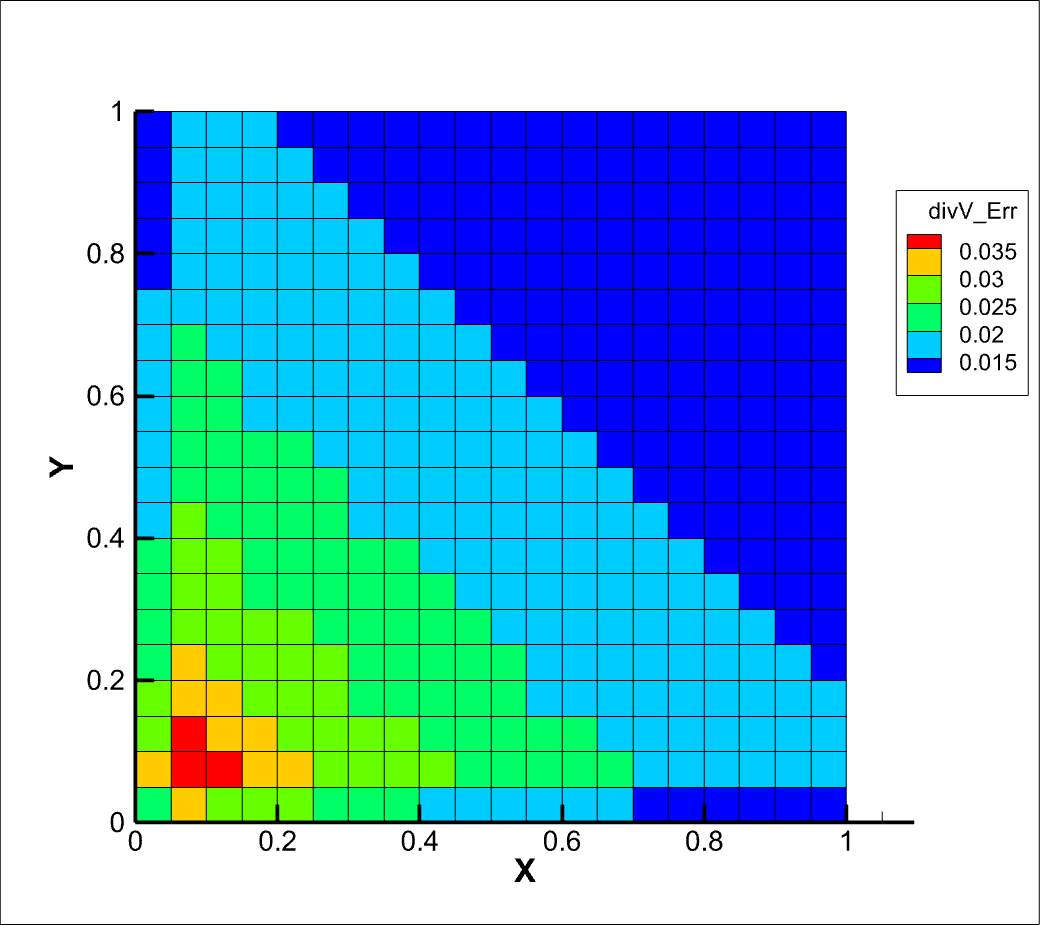
\includegraphics[width=0.3\textwidth]{img/19.2.png}}
    \subcaptionbox{SOU}{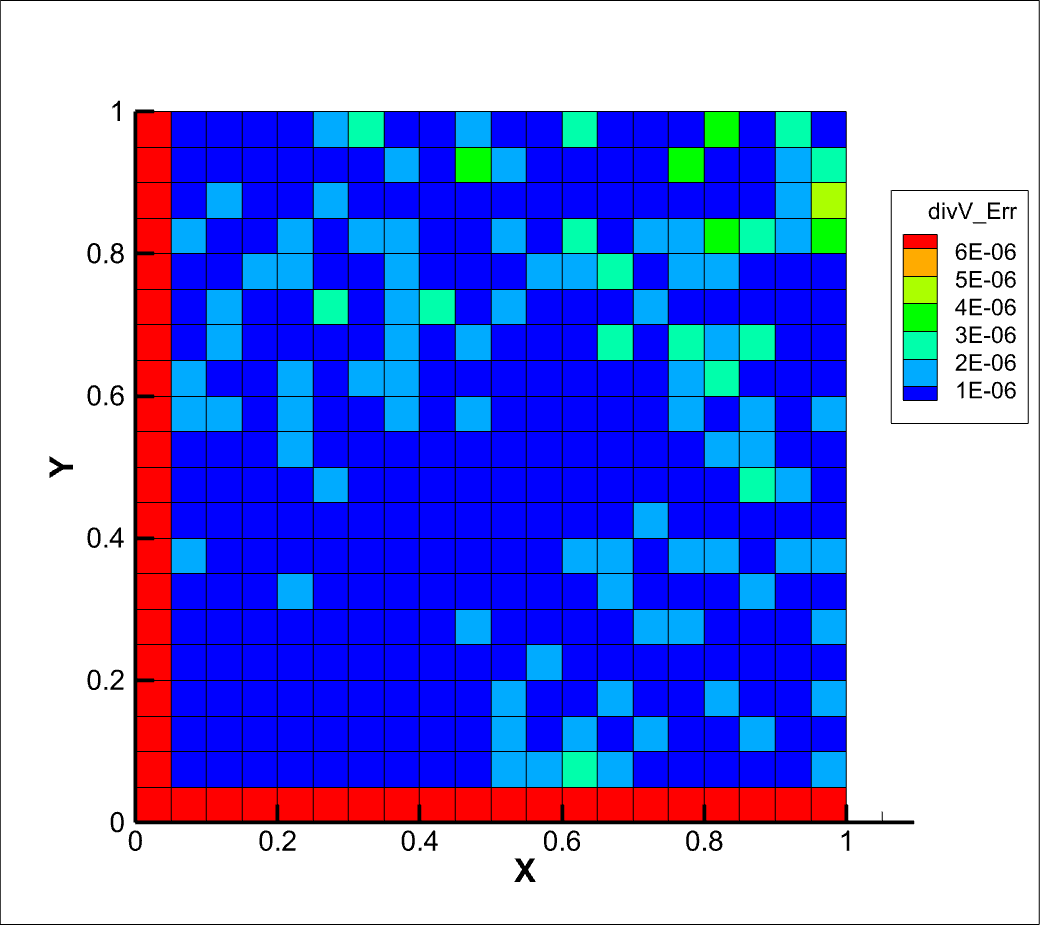
\includegraphics[width=0.3\textwidth]{img/19.3.png}}
    \caption{Распределение ошибки для полинома второй степени на base сетке.}
    \label{fig:19}
\end{figure}
Исходя из представленных на рисунках распределений видно, что для
полинома первой степени все рассмотренные схемы дают правильные с точностью до
машинной погрешности результаты. В случае полинома второй степени для
противопоточной схемы первого порядка возникает существенная ошибка во всей области,
а для Central и SOU во внутренней области по-прежнему наблюдается машинная точность.
Единственное, что схема SOU для второго ряда ячеек дает ошибку, превосходящую
машинную, что обусловлено ошибкой при расчете градиента в приграничных ячейках.
Рассмотрим распределения ошибки при расчетах на базовой и
измельченной сетках для полинома третьей степени.



\begin{figure}[H]
    \centering
    \subcaptionbox{Central}{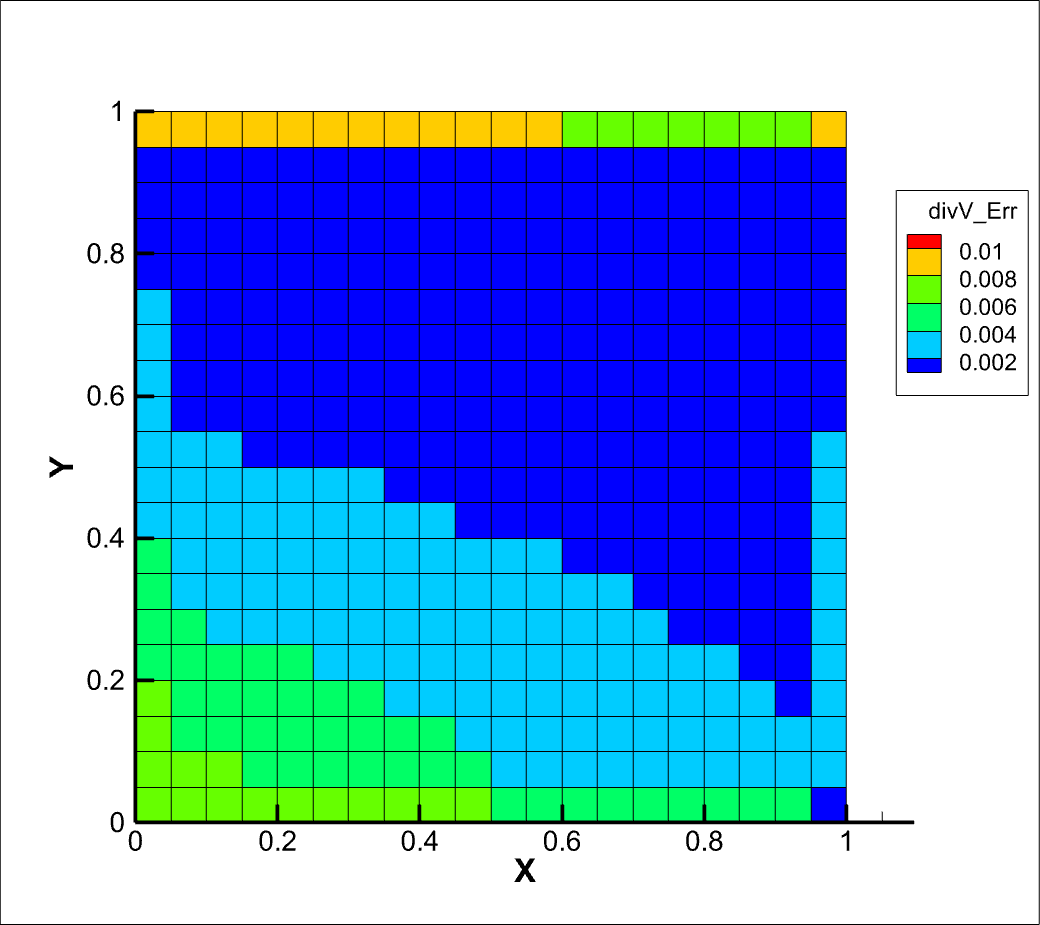
\includegraphics[width=0.3\textwidth]{img/20.1.png}}
    \subcaptionbox{FOU}{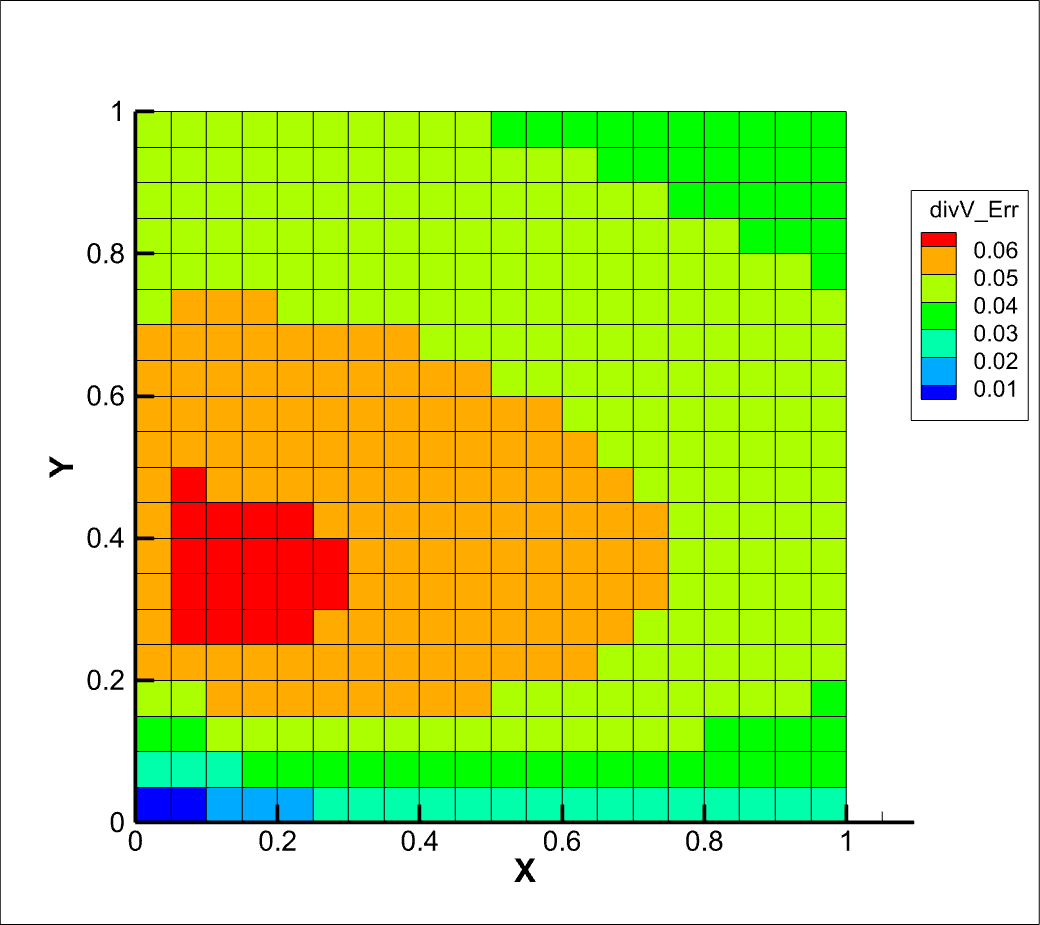
\includegraphics[width=0.3\textwidth]{img/20.2.png}}
    \subcaptionbox{SOU}{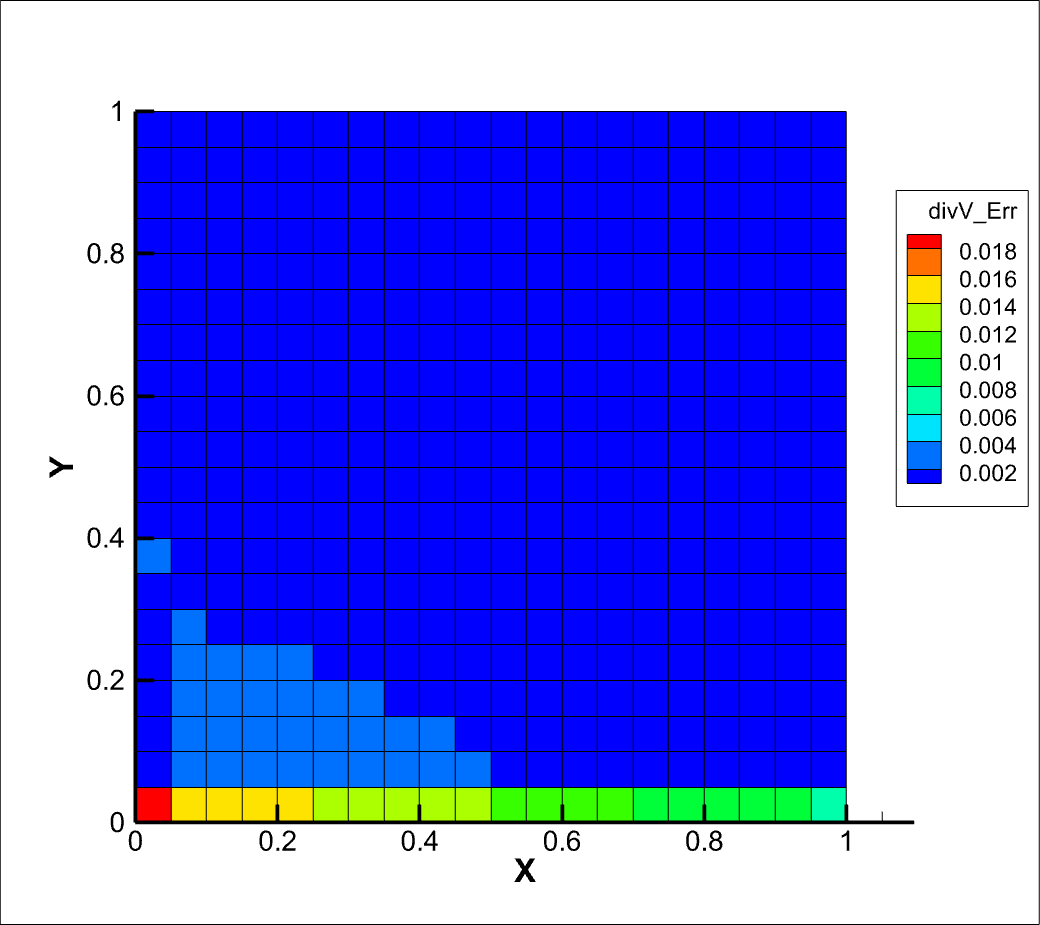
\includegraphics[width=0.3\textwidth]{img/20.3.png}}
    \caption{Распределение ошибки для полинома третьей степени на base сетке.}
    \label{fig:20}
\end{figure}

\begin{figure}[H]
    \centering
    \subcaptionbox{Central}{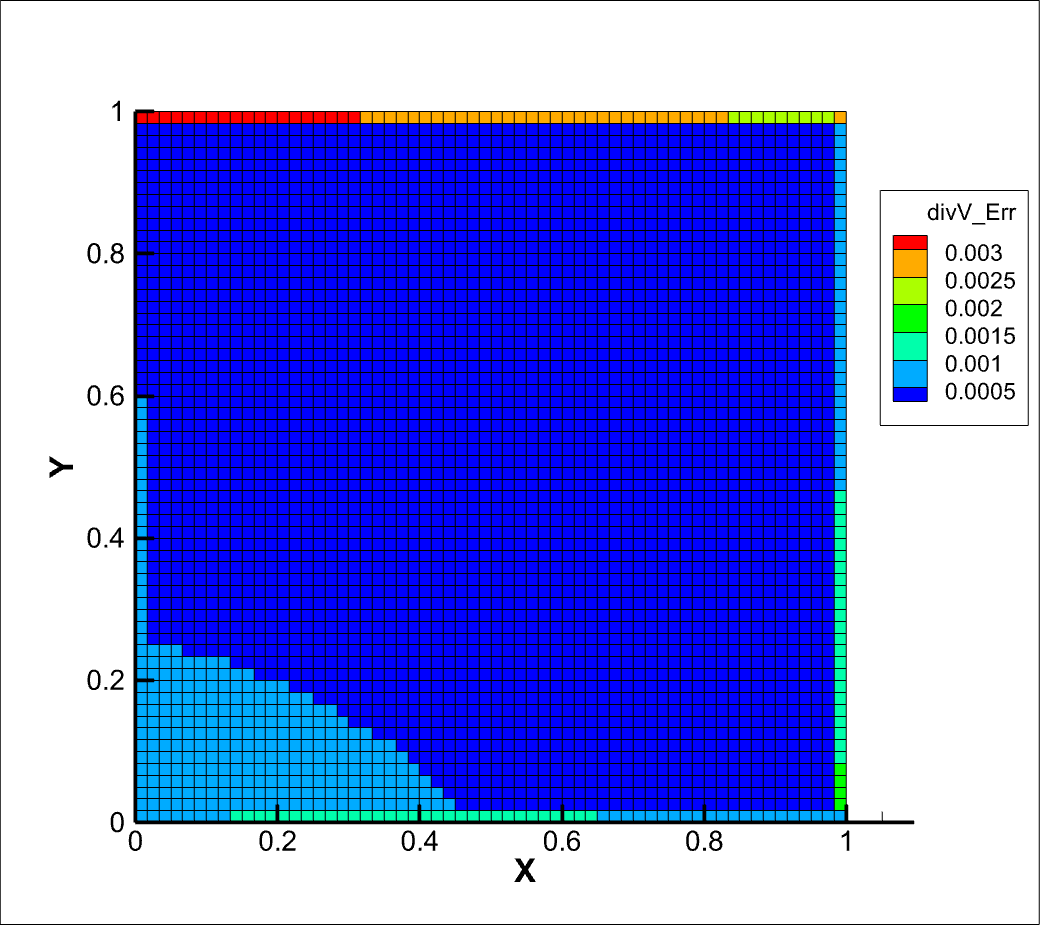
\includegraphics[width=0.3\textwidth]{img/21.1.png}}
    \subcaptionbox{FOU}{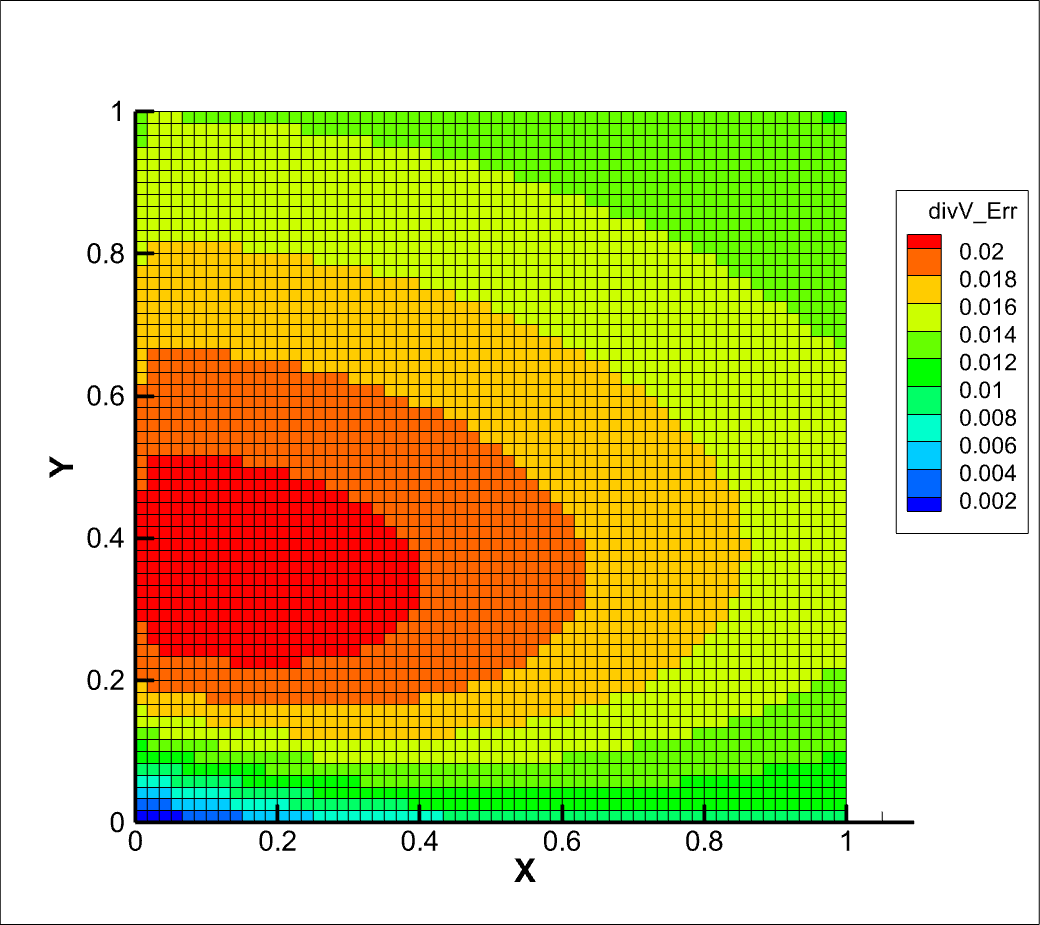
\includegraphics[width=0.3\textwidth]{img/21.2.png}}
    \subcaptionbox{SOU}{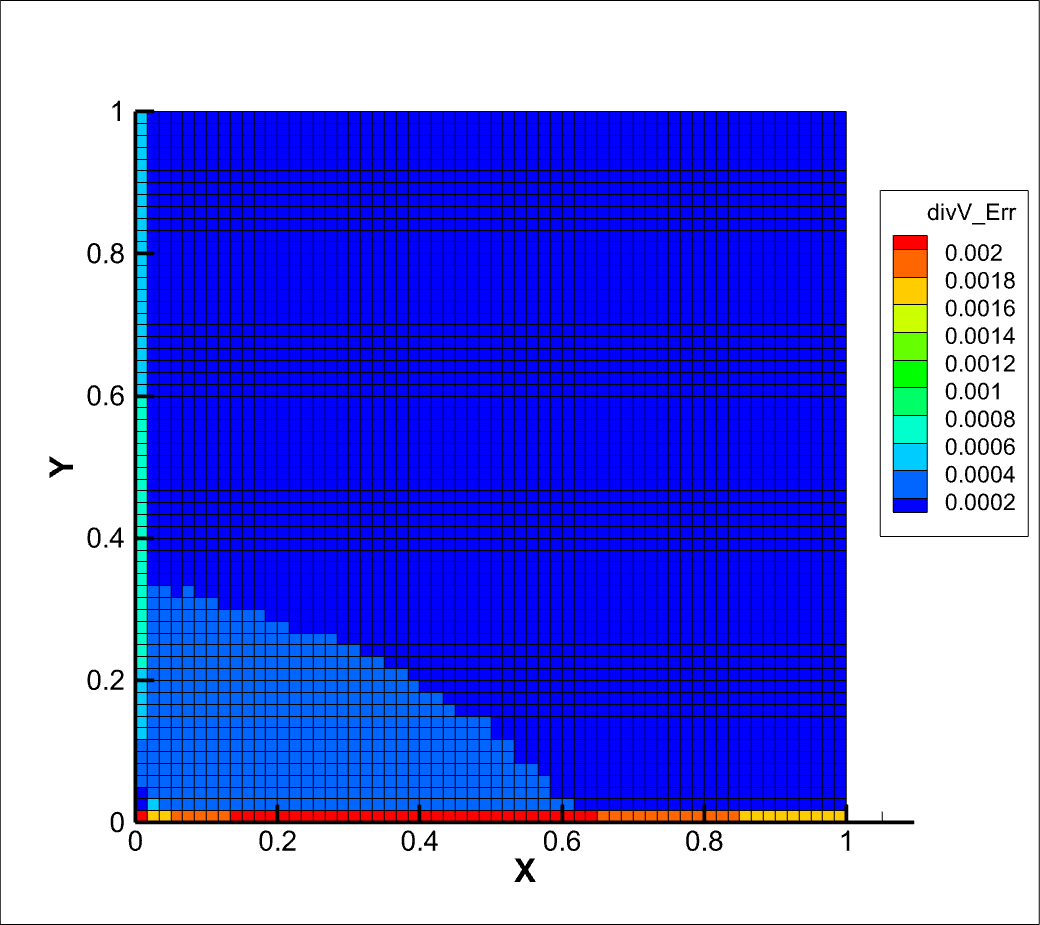
\includegraphics[width=0.3\textwidth]{img/21.3.png}}
    \caption{Распределение ошибки для полинома третьей степени на fine сетке.}
    \label{fig:21}
\end{figure}


По рисунку \ref{fig:22} можно заметить, что для схем Central, FOU и SOU (GG)
наблюдается очень большая ошибка уже для полинома D1, так как в них
отсутствует какая-либо поправка на скошенность.


\begin{figure}[H]
    \centering
    \subcaptionbox{Central}{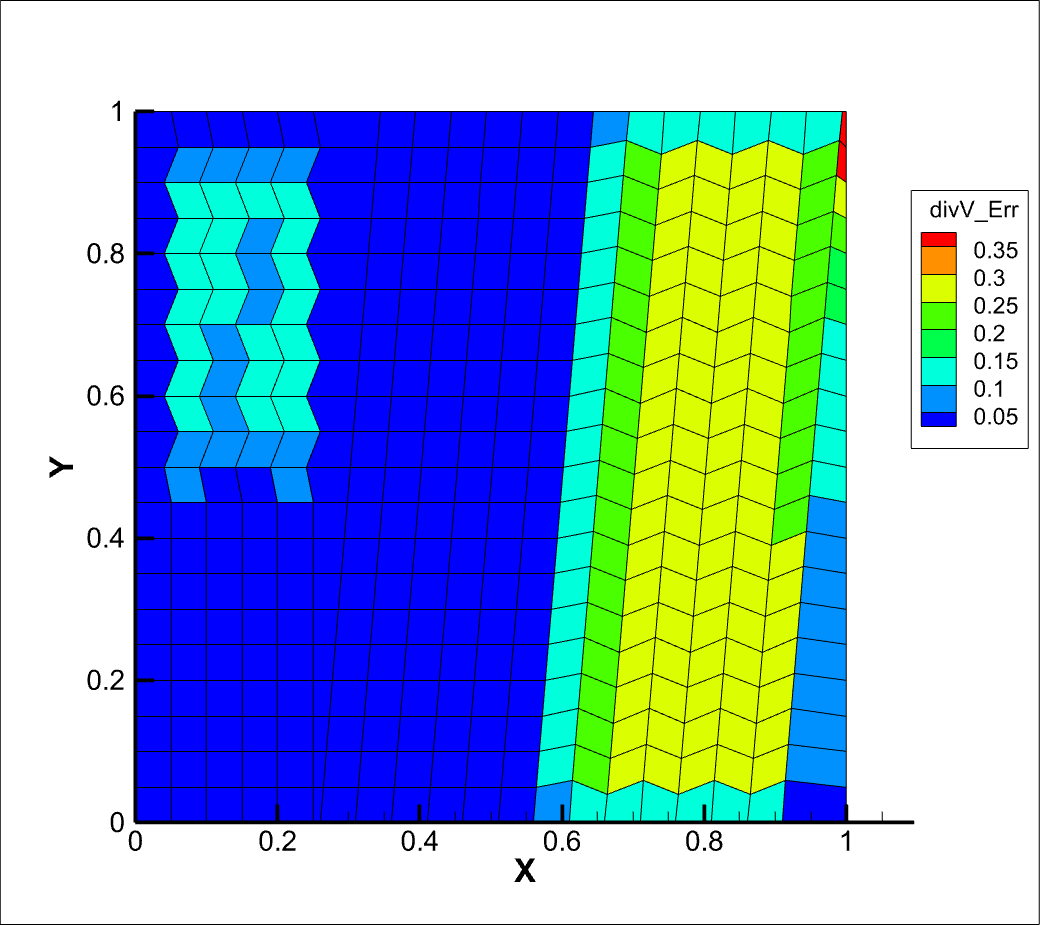
\includegraphics[width=0.3\textwidth]{img/22.1.png}}
    \subcaptionbox{FOU}{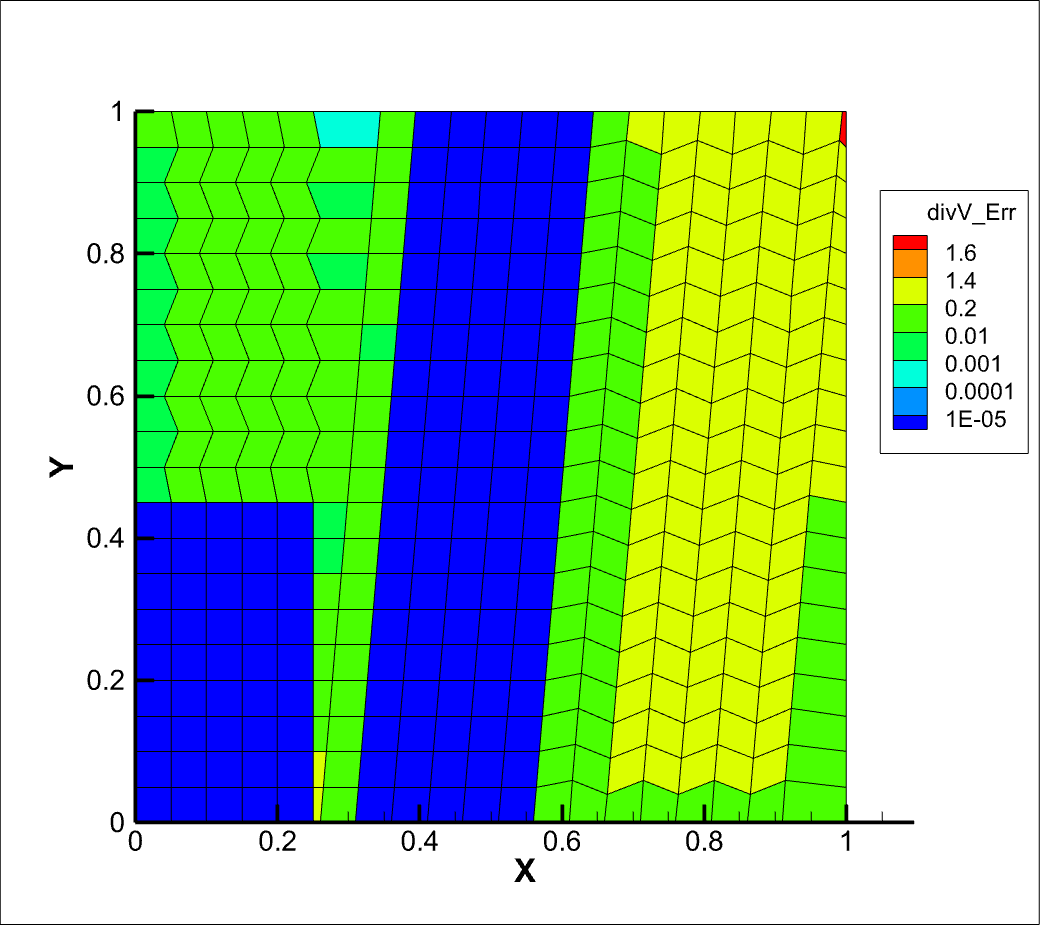
\includegraphics[width=0.3\textwidth]{img/22.2.png}}
    \subcaptionbox{SOU}{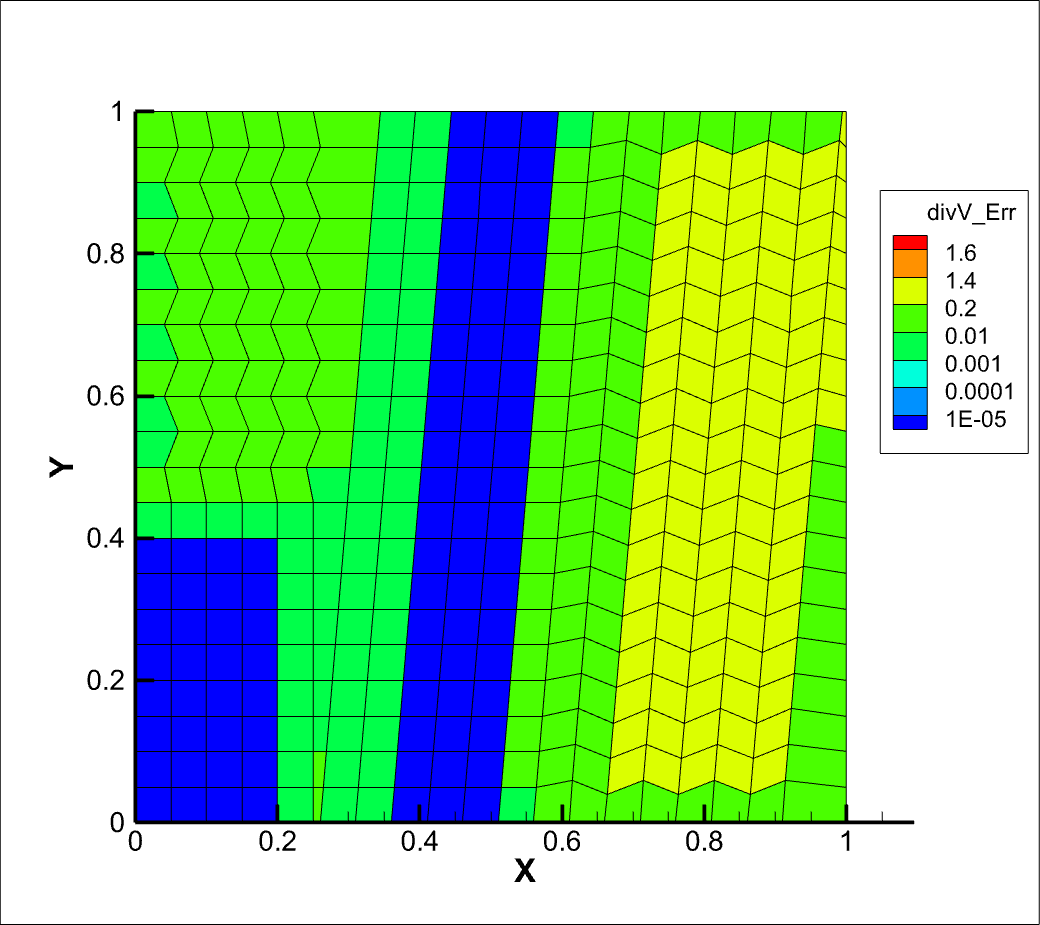
\includegraphics[width=0.3\textwidth]{img/22.3.png}}
    \caption{Распределение ошибки для полинома первой степени на skew сетке.}
    \label{fig:22}
\end{figure}

\subsection{Лапласиан скалярного поля.}

Рассчитаем лапласиан скалярного поля при помощи двух методов расчета градиента. В таблице \ref{tab:5} приведены значения относительной ошибки расчетов, как максимальная, так и в центре расчетной области.

\begin{table}[H]
    \centering
    \caption{Ошибка вычислений лаплсиана для различных методов и схем}
    \resizebox{\textwidth}{!}{%
    \begin{tabular}{|cc|cc|cc|}
    \hline
    \multicolumn{2}{|c|}{} &
      \multicolumn{2}{c|}{GG} &
      \multicolumn{2}{c|}{GGI} \\ \hline
    \multicolumn{1}{|c|}{Вид сетки} &
      P &
      \multicolumn{1}{c|}{max(Error)} &
      Error в центре &
      \multicolumn{1}{c|}{max(Error)} &
      Error в центре \\ \hline
    \multicolumn{1}{|c|}{} &
      P2 &
      \multicolumn{1}{c|}{8.32e-2} &
      3.15e-5 &
      \multicolumn{1}{c|}{2.78e-4} &
      3.11e-5 \\ \cline{2-6} 
    \multicolumn{1}{|c|}{} &
      P3 &
      \multicolumn{1}{c|}{0.29} &
      5.92e-6 &
      \multicolumn{1}{c|}{0.3} &
      5.43e-6 \\ \cline{2-6} 
    \multicolumn{1}{|c|}{\multirow{-3}{*}{Base}} &
      P4 &
      \multicolumn{1}{c|}{0.1} &
      9.6e-4 &
      \multicolumn{1}{c|}{1.42e-2} &
      9.9e-4 \\ \hline
    \multicolumn{1}{|c|}{Fine} &
      P4 &
      \multicolumn{1}{c|}{8.9e-2} &
      1.2e-4 &
      \multicolumn{1}{c|}{4.58e-3} &
      1.19e-4 \\ \hline
    \multicolumn{1}{|c|}{} &
      P2 &
      \multicolumn{1}{c|}{17.4} &
      \cellcolor[HTML]{9B9B9B} &
      \multicolumn{1}{c|}{8.37} &
      \cellcolor[HTML]{9B9B9B} \\ \cline{2-6} 
    \multicolumn{1}{|c|}{\multirow{-2}{*}{Skew}} & P3 & \multicolumn{1}{c|}{38.7} & \cellcolor[HTML]{9B9B9B} & \multicolumn{1}{c|}{16.7} & \cellcolor[HTML]{C0C0C0} \\ \hline
    \end{tabular}%
    }

    \label{tab:5}
\end{table}

Определим порядок точности для приграничной и внутренней ячеек:

\begin{itemize}
    \item GG: $O(\Delta p)_b = 0.1$, $O(\Delta p)_i = 1.89$
    \item GGI: $O(\Delta p)_b = 1.02$, $O(\Delta p)_i = 1.92$
\end{itemize}



На рисунка \ref{fig:23} - \ref{fig:28} представлены распределение ошибки в расчетной области для разных методов и видов полиномов.




\begin{figure}[H]
    \centering
    \subcaptionbox{GG}{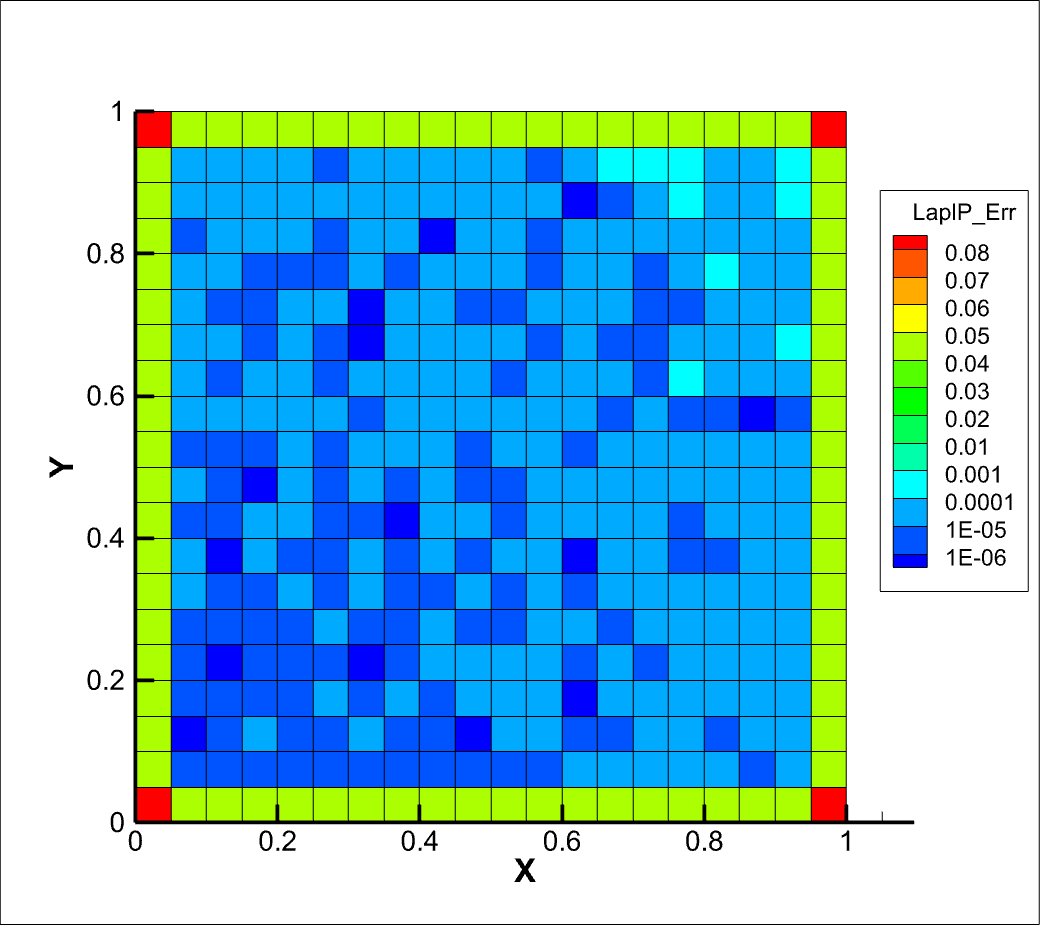
\includegraphics[width=0.45\textwidth]{img/23.1.png}}
    \subcaptionbox{GG with iteration}{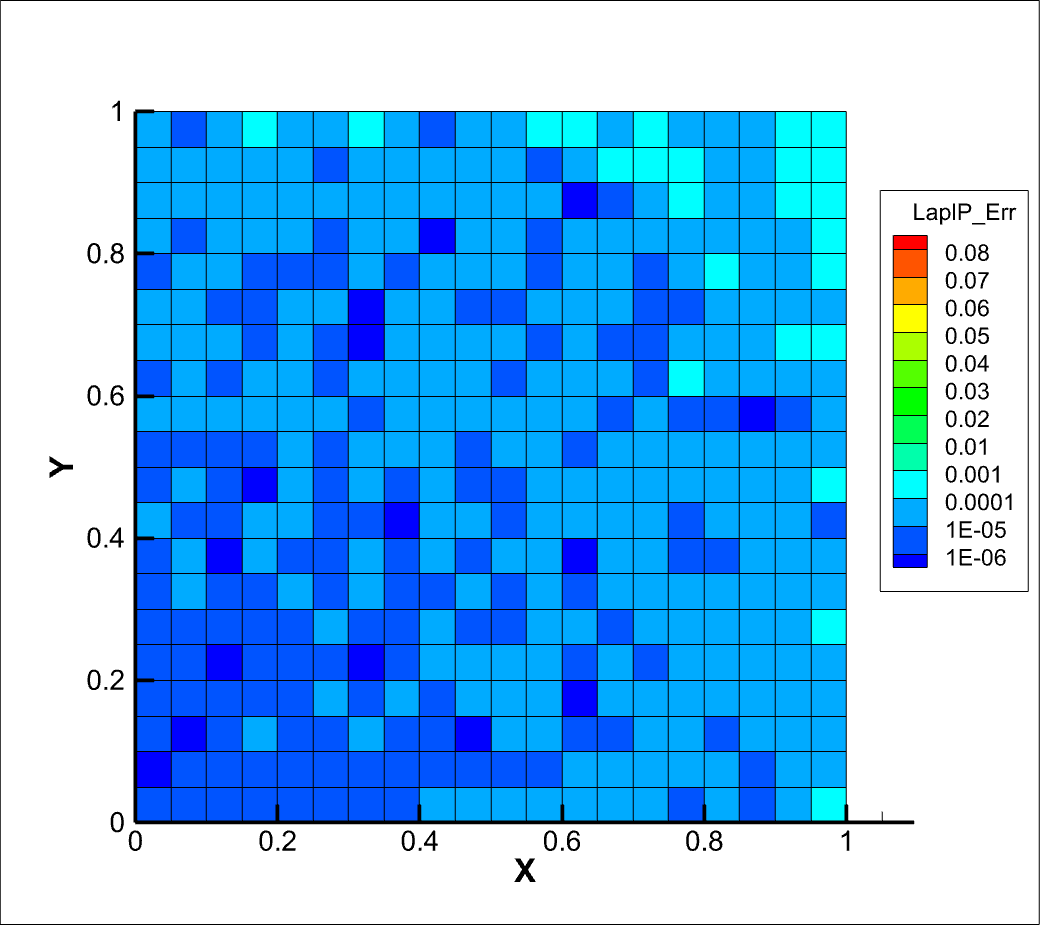
\includegraphics[width=0.45\textwidth]{img/23.2.png}}
    \caption{Распределение ошибки вычисления лапласиана для полинома второй степени на base сетке.}
    \label{fig:23}
\end{figure}
По рисунку \ref{fig:23} видно, что для метода GG в приграничных ячейках
наблюдается сильное увеличение погрешности, связанное со специальным
способом расчета градиента на границе. Во внутренней области для GG
наблюдается хаотическое поведение ошибки, однако её значение превышает
машинную точность. В случае метода GGI ошибка распределена хаотично уже
во всей области.

\begin{figure}[H]
    \centering
    \subcaptionbox{GG}{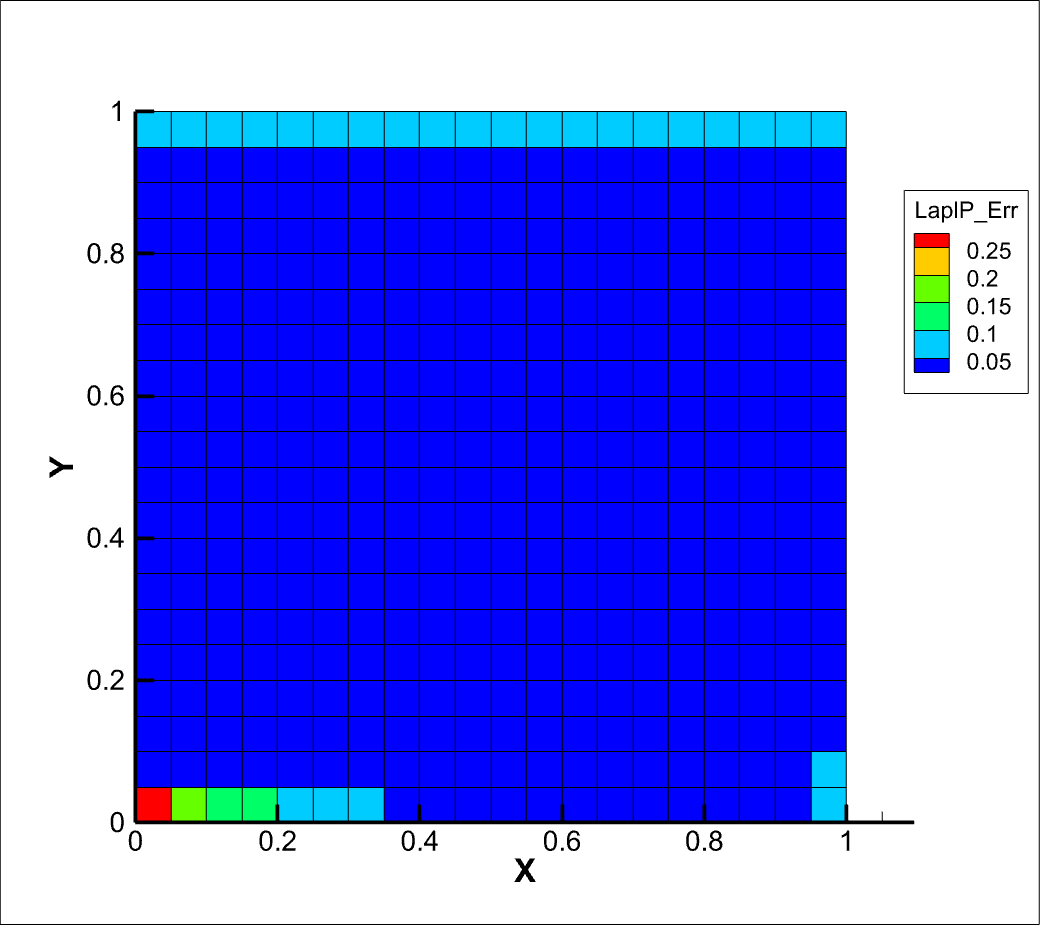
\includegraphics[width=0.45\textwidth]{img/24.1.png}}
    \subcaptionbox{GG with iteration}{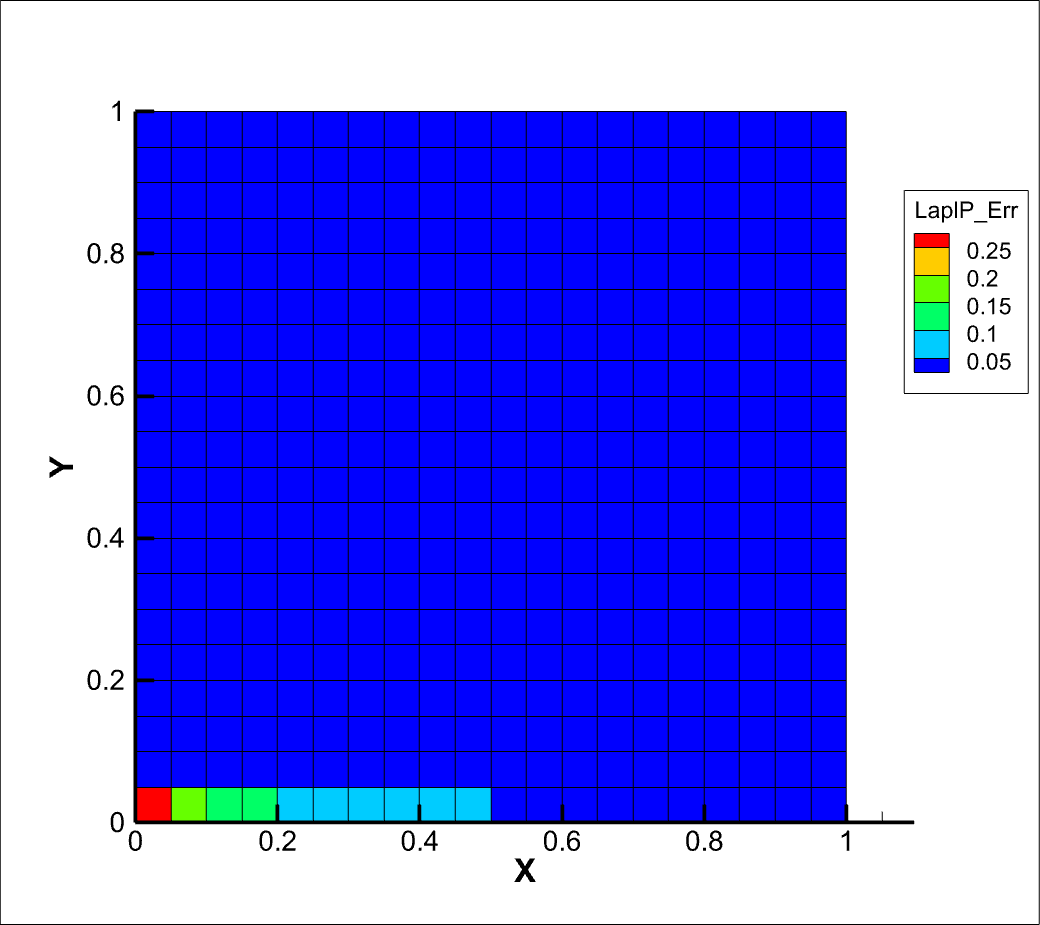
\includegraphics[width=0.45\textwidth]{img/24.2.png}}
    \caption{Распределение ошибки вычисления лапласиана для полинома третьей степени на base сетке.}
    \label{fig:24}
\end{figure}

Из рисунков \ref{fig:25} и \ref{fig:26} наблюдаем аналогичное поведение как и в предыдущих расчетах при измельчении сетки, что ошибка в центре сильно падает, и остается только на границах расчетной облсти.
\begin{figure}[H]
    \centering
    \subcaptionbox{GG}{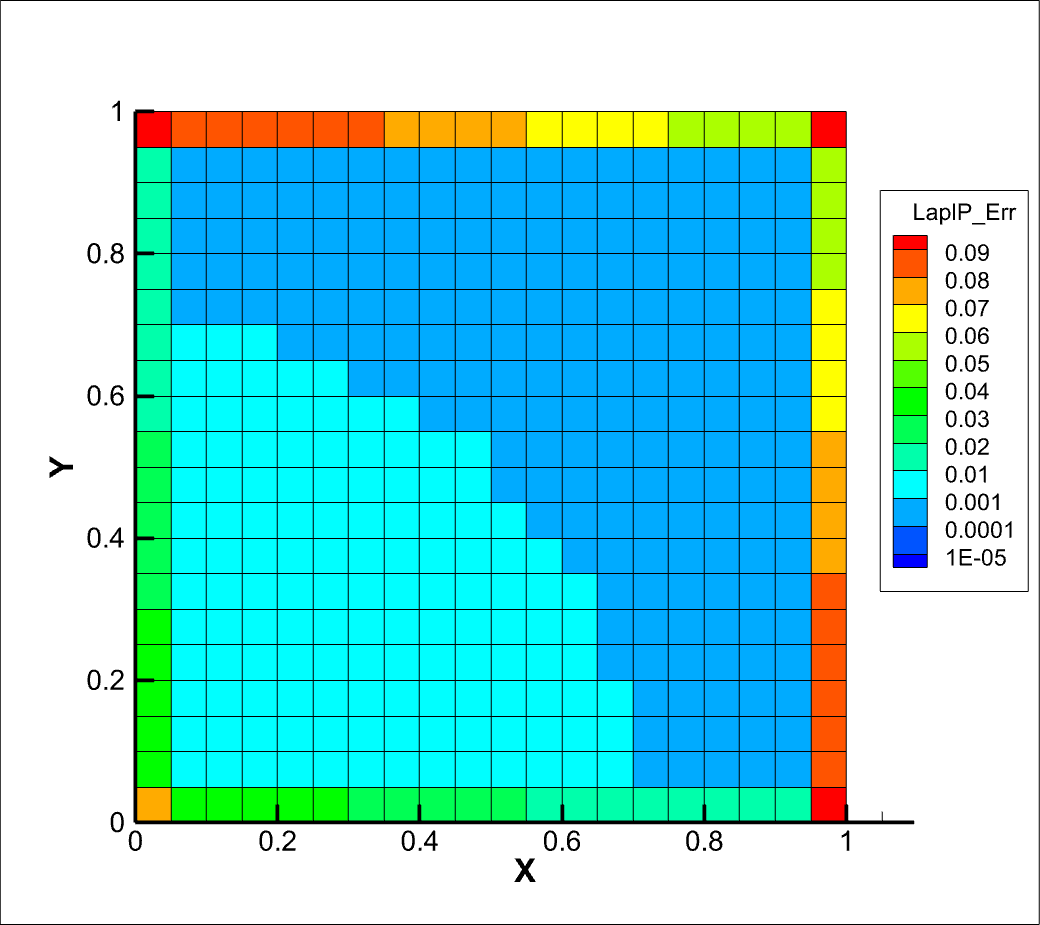
\includegraphics[width=0.45\textwidth]{img/25.1.png}}
    \subcaptionbox{GG with iteration}{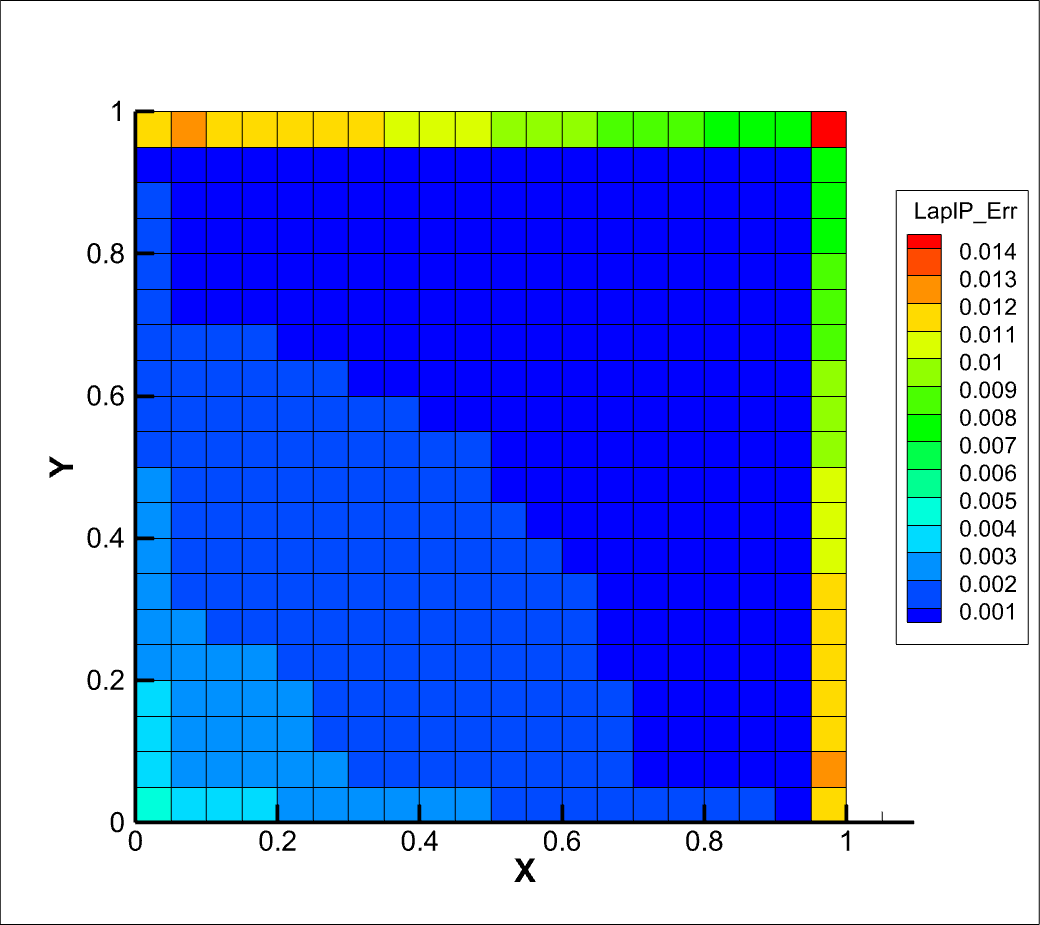
\includegraphics[width=0.45\textwidth]{img/25.2.png}}
    \caption{Распределение ошибки вычисления лапласиана для полинома четвертой степени на base сетке.}
    \label{fig:25}
\end{figure}

\begin{figure}[H]
    \centering
    \subcaptionbox{GG}{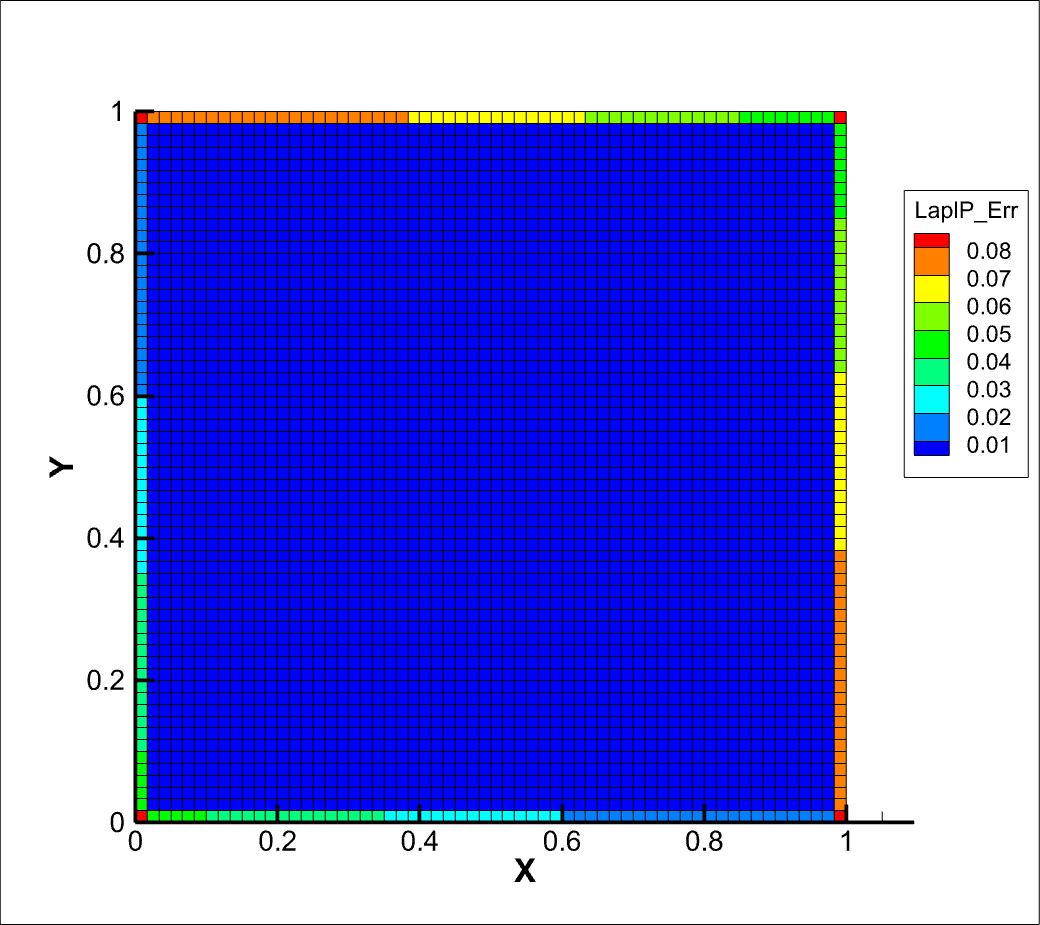
\includegraphics[width=0.45\textwidth]{img/26.1.png}}
    \subcaptionbox{GG with iteration}{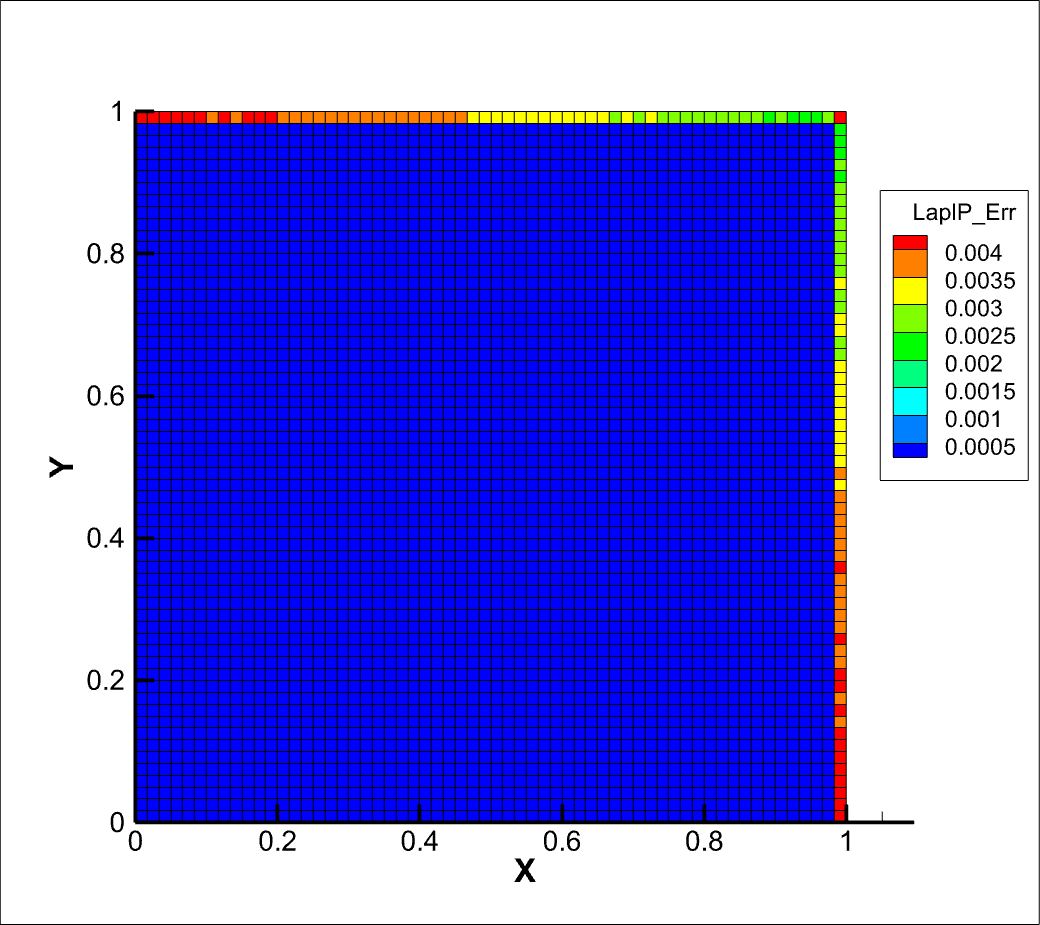
\includegraphics[width=0.45\textwidth]{img/26.2.png}}
    \caption{Распределение ошибки вычисления лапласиана для полинома второй степени на fine сетке.}
    \label{fig:26}
\end{figure}

\begin{figure}[H]
    \centering
    \subcaptionbox{GG}{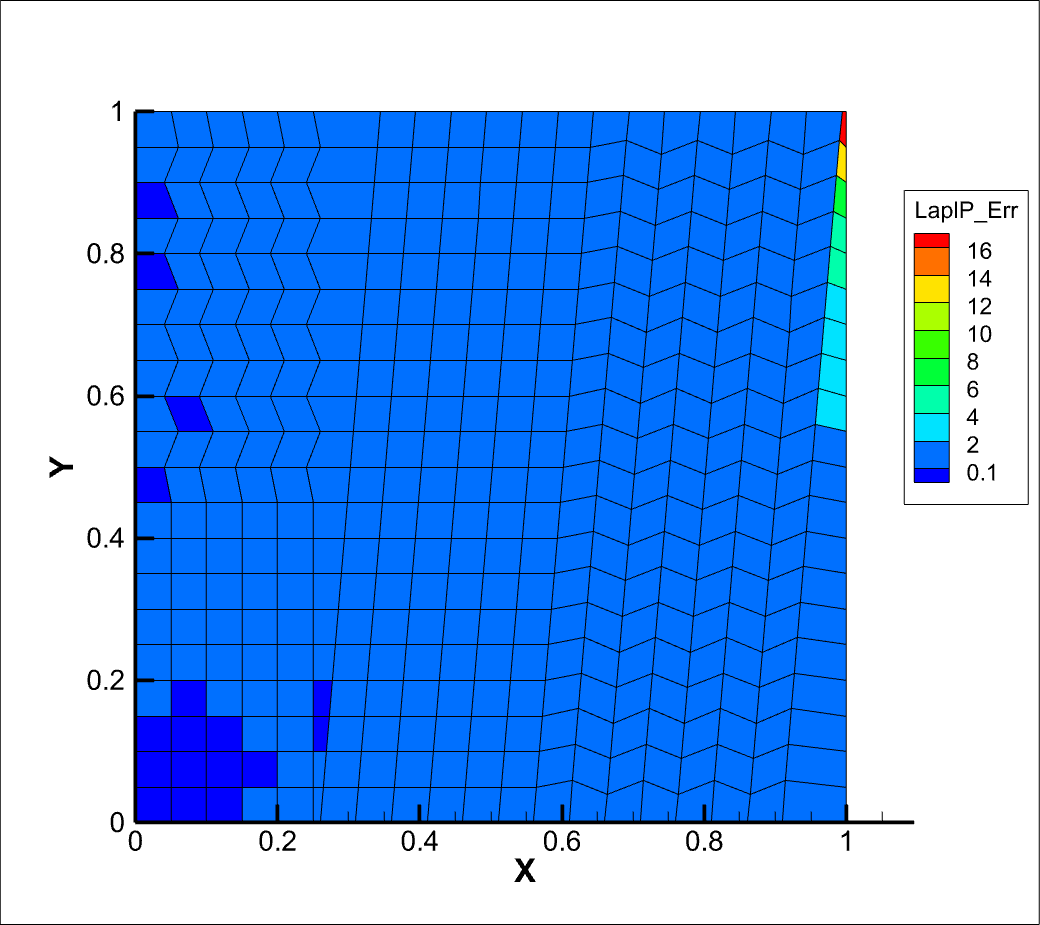
\includegraphics[width=0.45\textwidth]{img/27.1.png}}
    \subcaptionbox{GG with iteration}{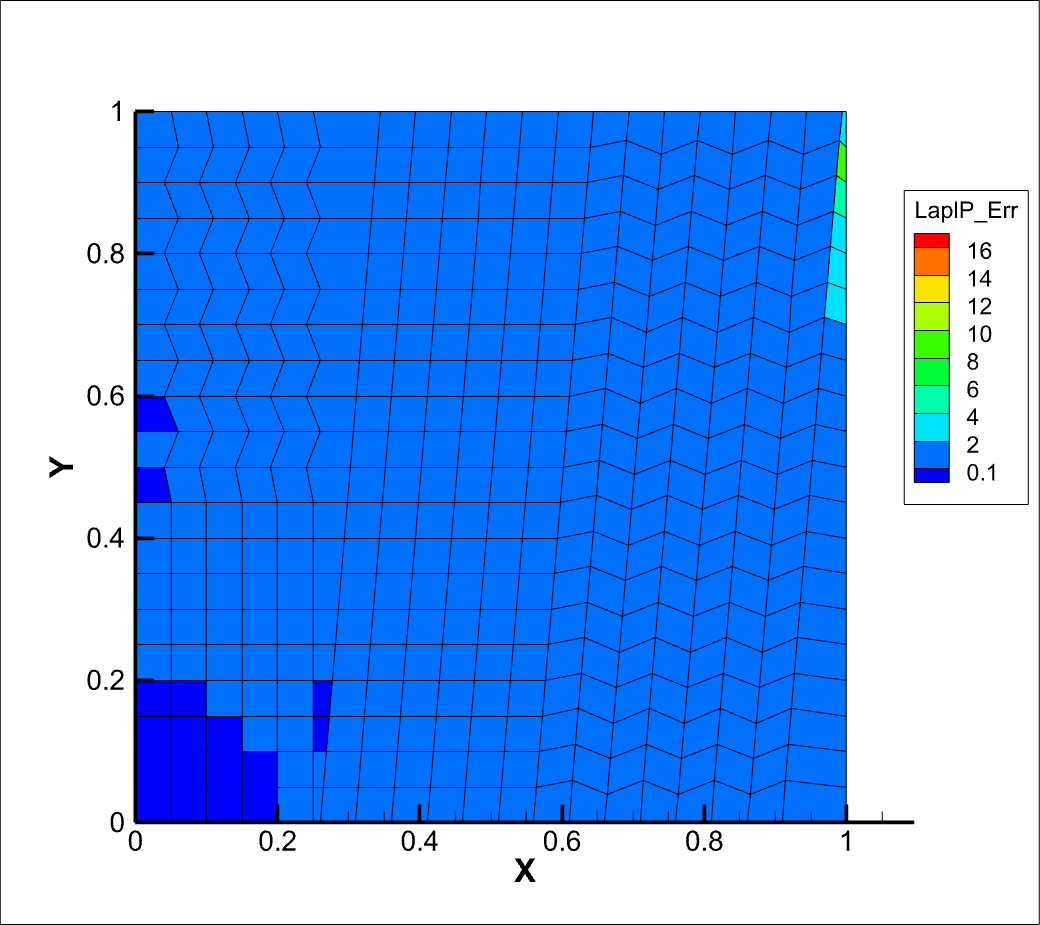
\includegraphics[width=0.45\textwidth]{img/27.2.png}}
    \caption{Распределение ошибки вычисления лапласиана для полинома второй степени на skew сетке.}
    \label{fig:27}
\end{figure}

\begin{figure}[H]
    \centering
    \subcaptionbox{GG}{\includegraphics[width=0.45\textwidth]{img/28.1.png}}
    \subcaptionbox{GG with iteration}{\includegraphics[width=0.45\textwidth]{img/28.2.png}}
    \caption{Распределение ошибки вычисления лапласиана для полинома третьей степени на skew сетке.}
    \label{fig:28}
\end{figure}


Для скошенных сеток наблюдаем огромные ошибки, которые уменьшаются при использовании итерационного метода.



\subsection{Расчет ротора векторного поля.}
Для расчета ротора векторного поля изпользовались полиномы третьей степени. Аналогично предыдущим трем пунктам. В таблице \ref{tab:6} представлены значения ошибки ротора как максимальной так и в центре расчетной области.


\begin{table}[H]
    \centering
    \caption{Ошибка вычислений ротора для различных сеток и полиномов}
    \resizebox{\textwidth}{!}{%
    \begin{tabular}{|c|cc|cc|cc|}
    \hline
       & \multicolumn{2}{c|}{Base}              & \multicolumn{2}{c|}{Fine}             & \multicolumn{2}{c|}{Skew}                               \\ \hline
    P & \multicolumn{1}{c|}{max(Error)} & Error в центре & \multicolumn{1}{c|}{max(Error)} & Error в центре & \multicolumn{1}{c|}{max(Error)} & Error в центре \\ \hline
    P1 & \multicolumn{1}{c|}{1.78e-6} & 4e-7    & \multicolumn{1}{c|}{7.39e-6} & 1e-7   & \multicolumn{1}{c|}{1e-1}    & \cellcolor[HTML]{C0C0C0} \\ \hline
    P2 & \multicolumn{1}{c|}{0.5}     & 5.25e-7 & \multicolumn{1}{c|}{0.5}     & 6e-7   & \multicolumn{1}{c|}{2.13}      & \cellcolor[HTML]{C0C0C0} \\ \hline
    P3 & \multicolumn{1}{c|}{8.5e-3}  & 1.2e-3  & \multicolumn{1}{c|}{2.9e-3}  & 1.3e-4 & \multicolumn{1}{c|}{7.69e-2} & \cellcolor[HTML]{C0C0C0} \\ \hline
    \end{tabular}%
    }

    \label{tab:6}
\end{table}
Оценим порядок точности для приграничной и внутренней ячеек соответственно:

\begin{itemize}
    \item $O(\Delta p)_b = 0.978$, $O(\Delta p)_i = 2.02$
\end{itemize}

На рисунка \ref{fig:29} - \ref{fig:31} представлены ошибки поля ротора. Можно заметить, что для полинома второй степени максимальная ошибка сильно выросла, это может быть связано с самим полиномом, а не сколько с методом. Для оплиномов первой степени для исходной и измельченной сеток наблюдаем машинную точность. Также и для полинома второй степени но внутри области. Для полинома третьей степени ошибка внутри стала больше.

\begin{figure}[H]
    \centering
    \subcaptionbox{P1}{\includegraphics[width=0.3\textwidth]{img/29.1.png}}
    \subcaptionbox{P2}{\includegraphics[width=0.3\textwidth]{img/29.2.png}}
    \subcaptionbox{P3}{\includegraphics[width=0.3\textwidth]{img/29.3.png}}
    \caption{Распределение ошибки ротора на base сетке.}
    \label{fig:29}
\end{figure}

\begin{figure}[H]
    \centering
    \subcaptionbox{P1}{\includegraphics[width=0.3\textwidth]{img/30.1.png}}
    \subcaptionbox{P2}{\includegraphics[width=0.3\textwidth]{img/30.2.png}}
    \subcaptionbox{P3}{\includegraphics[width=0.3\textwidth]{img/30.3.png}}
    \caption{Распределение ошибки ротора на fine сетке.}
    \label{fig:30}
\end{figure}

\begin{figure}[H]
    \centering
    \subcaptionbox{P1}{\includegraphics[width=0.3\textwidth]{img/31.1.png}}
    \subcaptionbox{P2}{\includegraphics[width=0.3\textwidth]{img/31.2.png}}
    \subcaptionbox{P3}{\includegraphics[width=0.3\textwidth]{img/31.3.png}}
    \caption{Распределение ошибки ротора на skew сетке.}
    \label{fig:31}
\end{figure}

Поскольку при расчете ротора не использовались никакие поправки на скошенность,
наблюдается существенная погрешность для большинства ячеек, а для полинома второй
степени погрешность больше, чем для первой степени.


\section{Перенос температуры в каверне.}

\subsection{Постановка задачи.}
В данной работе проводится численное решение уравнения
конвективно-диффузионного переноса температуры в заданном поле
скоростей по МКО, применительно к задаче о течении в каверне с движущейся
крышкой и с разнонагретыми стенками.
Каверна имеет две изотермические стенки левая - горячая, правая - холодная, температура холодной стенки $T_cold$ равна 1.0, температура горячей стенки $T_hot$ равна 2.0. Две другие стенки каверны – адиабатические. Задача решается в безразмерной постановке, масштабы для обезразмеривания задачи: H – высота каверны, $U_w=1$ – скорость движения крышки (верхней стенки) каверны. Течение и теплообмен в каверне определяются следующими безразмерными параметрами: K = L/H = 0.5 – геометрический фактор (отношение ширины L каверны к ее высоте H), Re=90 – число Рейнольдса, Pr=1 – число Прандтля. Расчетная область и сетка представлены на рисунке \ref{fig:32}.

\begin{figure}[H]
    \centering
    \includegraphics[width=0.55\textwidth]{img/32.png}
    \caption{Вид расчетной области.}
    \label{fig:32}
\end{figure}

В данном случае используется скошенная регулярная сетка, состоящая из прямоугольников. Граничные условия представлены на рисунке \ref{fig:33}.

\begin{figure}[H]
    \centering
    \includegraphics[width=0.55\textwidth]{img/33.png}
    \caption{Граничные условия.}
    \label{fig:33}
\end{figure}

Для нахождения численного решения был написан дополнительный модуль под названием B\_CalcResT. Он представляет из себя возможность проведения расчетов конвективных и диффузионных потоков на гранях вследствии чего находятся невязки и значения шагов по псевдовремени. Также он учитывается нулевой тепловой поток на нижней и верхней стенке. Для достижения эффекта адиабатической стенки на каждой итерации значение температуры в фиктивных ячейках меняется таким образом, чтобы на грани градиент температуры вдоль нормали к грани был равен нулю.

Также в работе необходимо выполнить расчет в ПО Flos и сравнить полученные результаты с вычисленными.

\subsection{Результаты полученны с помощью программы FLOS.}
Сетка строилась в программе FLOS и имеет размеры 21x21 ячейки. На рисунке \ref{fig:01} изображено поле модуля скорости, линии тока, а также поле температуры.
\begin{figure}[H]
    \centering
    \subcaptionbox{Поле модуля скорости.}{\includegraphics[width=0.3\textwidth]{img/01.1.png}}
    \subcaptionbox{Поле температуры.}{\includegraphics[width=0.3\textwidth]{img/01.2.png}}
    \subcaptionbox{Линии тока.}{\includegraphics[width=0.3\textwidth]{img/01.3.png}}
    \caption{Поля распределений величин.}
    \label{fig:01}
\end{figure}
Видно, что большие скорости достигаются в верхней части каверны в частности в правом верхнем углу. Как видно, так как верхняя крышка каверны находится в
движении, образуется круговое движение жидкости по часовой стрелке в
верхней половине каверны, что подтверждает картина распределения линий
тока, где можно заметить, что в верхней половине каверны
образуется один большой вихрь, а в нижней появляется еще один но менее интенсивный с меньшими скоростями.

В свою очередь в можно увидеть, что наличие конвективного
переноса приводит к искажению изолиний температуры. Наибольшее
искажение изолиний наблюдается в области основного вихря. При этом на
нижней стенке изолинии практически вертикальные, что согласуется с
поставленным условием адиабатичности на ней. На верхней стенке также
поставлено условие адиабатичности, однако из-за движения данной границы
изолинии температуры искажаются в сторону движения стенки.

В таблице \ref{tab:9} представлены входные параметры, задаваемые для получения решения. Значения чисел Куранта и фон Неймана задавались таким образом, чтобы добиться максимальной устойчивости.



\begin{table}[H]
    \centering
    \caption{Входные параметры}
    \resizebox{0.3\textwidth}{!}{%
    \begin{tabular}{|c|c|}
    \hline
    Входной параметр                  & Значение    \\ \hline
    Метод расчета $\nabla T$                 & GGI         \\ \hline
    Cхема расчета конв. потоков       & Central UGB \\ \hline
    $V_s$, м/с                       & 1           \\ \hline
    $L_s$, м                         & 0.5         \\ \hline
    $Re$                              & 90          \\ \hline
    $Pr$                           & 1           \\ \hline
    $CFL$                           & 1           \\ \hline
    $VNM$                           & 0.03        \\ \hline
    Количество итераций (niter)  & 15000       \\ \hline
    \end{tabular}%
    }

    \label{tab:9}
\end{table}
Как говорилось ранее, наличие конвективных поток приводит к
искажению изолиний температуры. Для наглядности в ходе исследования с
помощью вычислительного кода был проведен расчет в случае отсутствия
конвективных потоков на расчетной сетке, полученной в программе Flos. Поле
температуры в случае такой постановки задачи представлено на рисунке \ref{fig:02}.

\begin{figure}[H]
    \centering
    \includegraphics[width=0.75\textwidth]{img/02.png}
    \caption{Поле температуры в отсутствие конвекции.}
    \label{fig:02}
\end{figure}

Видно, что в данном случае температура меняется линейно от значения 1 до 2.

При решении задачи в случае наличия конвективных потоков были получены графики истории сходимости, представленные на рисунке \ref{fig:03}.

\begin{figure}[H]
    \centering
    \includegraphics[width=0.75\textwidth]{img/03.png}
    \caption{График невязок.}
    \label{fig:03}
\end{figure}


Для обеих схем были определены максимальные значеня ошибки:

\begin{itemize}
    \item Central : $Error(T)_{max} = 3.78E-02$
    \item UGB: $Error(T)_{max} = 4.26E-02$
\end{itemize}


На рисунке \ref{fig:04} представлены распределения ошибки при исользовании различных схем. 

\begin{figure}[H]
    \centering
    \subcaptionbox{Central}{\includegraphics[width=0.45\textwidth]{img/04.1.png}}
    \subcaptionbox{UGB}{\includegraphics[width=0.45\textwidth]{img/04.2.png}}
    \caption{Распределение ошибки температуры.}
    \label{fig:04}
\end{figure}

Видно, что для схемы Upwind Gradine Based ошибка чуть больше чем для центрально-разностной схемы, однако отличия качественные в температурном поле не велики, потому будут представлены пол только для Central схемы.

\begin{figure}[H]
    \centering
    \subcaptionbox{FLOS}{\includegraphics[width=0.45\textwidth]{img/05.1.png}}
    \subcaptionbox{Fortran}{\includegraphics[width=0.45\textwidth]{img/05.2.png}}
    \caption{Поле температуры.}
    \label{fig:05}
\end{figure}
Видно по рисунку \ref{fig:05} что поля совподают, а отклонения малы в существенной части расчетной области.
\begin{figure}[H]
    \centering
    \subcaptionbox{x - компонента}{\includegraphics[width=0.45\textwidth]{img/06.1.png}}
    \subcaptionbox{y - компонента}{\includegraphics[width=0.45\textwidth]{img/06.2.png}}
    \caption{Поля компонент градиента температуры.}
    \label{fig:06}
\end{figure}
Из рисунка \ref{fig:06} делаем вывод о том, что там где скорость максимально тепловой поток тоже максимален в тоже самое время поперечный тепловой поток изменяется не так существенно. Напомним что тепловой поток пропорционален и обратен по знаку градиенту температуры.

\subsection{Результаты тестирования эффективности параллелилзации.}
В данном пункте проводится исследование эффективности
параллелизации, реализованной с помощью технологии OpenMP. Запуск
программы проводился при схеме расчета конвективных слагаемых UGB. 
Для проведения исследования эффективности параллелизации часть программы,
задействованная при решении уравнения конвективно-диффузионного переноса
температуры, была параллелизована средствами OpenMP. Для этого была добавлена
директива OMP DO перед вложенным циклом по всем ячейкам в подпрограммах для
расчета градиента температуры и её невязки, которая является директивой
распараллеливания циклов, а именно она осуществляет автоматическое распределение
итераций циклу между нитями. Для оценки эффективности параллелизации задавалось
различное количество нитей от 1 до 4 с помощью переменной окружения
OMP\_NUM\_THREADS, а использование функции OMP\_GET\_WTIME позволяло
определять время работы параллельной области программы.


В таблице \ref{kon} приведена зависимость времени работы от количества используемых нитей и расчет ускорения и эффективности по следующим формулам:
$$S_p = T_1/T_p;~~~~~~E_p=S_p/p$$
, где $p$ - число нитей, а $T_1$ - время последоваельного выполнения программы.
% Please add the following required packages to your document preamble:
% \usepackage{graphicx}
\begin{table}[]
    \caption{Зависимость времени, ускорения и эффективности от количества нитей.}
    \centering
    \resizebox{0.3\textwidth}{!}{%
    \begin{tabular}{|c|c|c|c|}
    \hline
    p  & T, c & $S_p$ & $E_p$ \\ \hline
    1 & 75.8 & 1     & 1     \\ \hline
    2 & 41.4 & 1.81  & 0.91  \\ \hline
    3 & 33.4 & 2.24  & 0.75  \\ \hline
    4 & 27.4 & 2.74  & 0.68  \\ \hline
    8 & 20.3 & 3.69  & 0.46  \\ \hline
    \end{tabular}%
    }

    \label{tab:kon}
\end{table}
На рисунке \ref{fig:last} изображены графики зависимости ускорения и эффективности от количества нитей.

\begin{figure}[H]
    \centering
    \subcaptionbox{Ускорение}{\includegraphics[width=0.45\textwidth]{img/l1.png}}
    \subcaptionbox{Эффективность}{\includegraphics[width=0.45\textwidth]{img/l2.png}}
    \caption{Поля компонент градиента температуры.}
    \label{fig:last}
\end{figure}

Исходя из значений, приведенных в таблице \ref{kon}, и графиков видно, что
наблюдается довольно сильное отклонение от идеальных зависимостей, как для ускорения,
так и для эффективности, уже при p = 3 эффективность параллелизации отклонилась
примерно на 20\%, и с дальнейшим увеличением числа нитей отклоняется все сильнее. На графике эффективности можно наблюдать аналогичные
результаты: при трех ядрах $E_p$ падает практически на 25\%, после чего
эффективность также продолжает падать. Таким образом, в случае данной
постановки задачи распараллеливание неэффективно.

Проверим как влияют встроенные опции оптимизации в компиляторе gfortran. Расчет производились на 4 нитях.
\begin{itemize}
    \item O0: 27.62 c
    \item O1: 12.86 с
    \item O2: 12.56 с
\end{itemize}

Получим, что использование любой встроенной опции оптимизации компилятара автоматически ускоряет работу программу почти в два раза.

\section{Выводы.}
\begin{itemize}
    \item Проведено исследование численных методов для расчёта дифференциальных операторов на двумерных сетках с использованием метода конечных объёмов. Особое внимание уделено работе с различными типами структурированных сеток, включая скошенные. Для вычислений использовалась программа, реализованная на языке Fortran.

    \item В рамках исследования были изучены два метода расчёта градиента скалярного поля: Грина-Гаусса (GG) и его модификация GGI. Метод GG продемонстрировал второй порядок точности как внутри расчётной области, так и на границах, благодаря специальным алгоритмам обработки. Однако метод GGI, сохраняя второй порядок точности внутри области, обладает первым порядком точности на границах. Его основное преимущество заключается в возможности учитывать скошенность сеток, что позволило значительно снизить ошибки на таких геометриях.
    
    \item Расчёты дивергенции произведения скалярной функции и векторного поля выполнены с использованием схем Central, FOU и SOU. Схема Central показала второй порядок точности внутри расчётной области и первый на её границах. Схема FOU обеспечила второй порядок точности во всех ячейках. Схема SOU, аналогичная Central по точности, проявила себя лучше на скошенных сетках благодаря сочетанию с методом GGI.
    
    \item Рассчитан лапласиан скалярного поля, для которого градиент вычислялся методами GG и GGI. Лапласиан показал второй порядок точности во внутренних ячейках независимо от метода расчёта градиента. Однако в приграничных ячейках метод GG продемонстрировал точность ниже первого порядка, тогда как GGI обеспечил первый порядок и снизил ошибки на скошенных сетках.
    
    \item Также был рассчитан ротор векторного поля методом линейной интерполяции. Результаты показали второй порядок точности во внутренних ячейках и первый порядок на границах.
    
    \item Решено уравнение конвективно-диффузионного переноса температуры в задаче течения в каверне с движущейся крышкой и разнонагретыми стенками. Конвективные члены уравнения рассчитывались схемами Central и Upwind Gradient Based. Движение крышки вызвало формирование крупного вихря в верхней части каверны, что привело к искажению изолиний температуры. Схема UGB продемонстрировала менее точные результаты по сравнению с Central.
    
    \item Кроме того, проведено исследование эффективности параллелизации кода с использованием технологии OpenMP. Установлено, что ускорение при увеличении числа ядер отстаёт от линейного: при использовании двух ядер эффективность распараллеливания снизилась на 30\%, что указывает на ограничение возможностей параллельного выполнения для данной задачи.
    
    \item Наконец, проведён анализ времени выполнения программы при использовании различных флагов оптимизации. Оптимизации -O1 и -O2 позволили сократить время работы программы почти в два раза.
\end{itemize}